% This is the Duke University Statistical Science LaTeX thesis template.
% It has been adapted from the Reed College LaTeX thesis template. The
% adaptation was done by Mine Cetinkaya-Rundel (MCR). Some of the comments
% that are specific to Reed College have been removed.
%
% Most of the work on the original Reed College document class and template
% was done by Sam Noble (SN). Later comments etc. by Ben Salzberg (BTS).
% Additional restructuring and APA support by Jess Youngberg (JY).
%
% See https://www.reed.edu/cis/help/latex/ for help. There are a
% great bunch of help pages there, with notes on
% getting started, bibtex, etc. Go there and read it if you're not
% already familiar with LaTeX.
%
% Any line that starts with a percent symbol is a comment.
% They won't show up in the document, and are useful for notes
% to yourself and explaining commands.
% Commenting also removes a line from the document;
% very handy for troubleshooting problems. -BTS

%%
%% Preamble
%%
% \documentclass{<something>} must begin each LaTeX document
\documentclass[12pt,twoside]{dukestatscithesis}
% Packages are extensions to the basic LaTeX functions. Whatever you
% want to typeset, there is probably a package out there for it.
% Chemistry (chemtex), screenplays, you name it.
% Check out CTAN to see: http://www.ctan.org/
%%
\usepackage{graphicx,latexsym}
\usepackage{amsmath}
\usepackage{amssymb,amsthm}
\usepackage{longtable,booktabs,setspace}
\usepackage{chemarr} %% Useful for one reaction arrow, useless if you're not a chem major
\usepackage[hyphens]{url}
% Added by CII
\usepackage{hyperref}
\usepackage{lmodern}
\usepackage{float}
\floatplacement{figure}{H}
% End of CII addition
\usepackage{rotating}

% Next line commented out by CII
%%% \usepackage{natbib}
% Comment out the natbib line above and uncomment the following two lines to use the new
% biblatex-chicago style, for Chicago A. Also make some changes at the end where the
% bibliography is included.
%\usepackage{biblatex-chicago}
%\bibliography{thesis}


% Added by CII (Thanks, Hadley!)
% Use ref for internal links
\renewcommand{\hyperref}[2][???]{\autoref{#1}}
\def\chapterautorefname{Chapter}
\def\sectionautorefname{Section}
\def\subsectionautorefname{Subsection}
% End of CII addition

% Added by CII
\usepackage{caption}
\captionsetup{width=5in}
% End of CII addition

% \usepackage{times} % other fonts are available like times, bookman, charter, palatino


% To pass between YAML and LaTeX the dollar signs are added by CII
\title{Statistical Analysis of the Human Gut Microbiome}
\author{Vivek Sriram}
% The month and year that you submit your FINAL draft TO THE LIBRARY (May or December)
\date{May 2019}
\advisor{Li Ma}
\institution{Duke University}
\degree{Bachelor of Science in Statistical Science}
\committeememberone{Alexander Volfovsky}
\committeemembertwo{Fan Li}
\dus{Amy Herring}
%If you have two advisors for some reason, you can use the following
% Uncommented out by CII
% End of CII addition

%%% Remember to use the correct department!
\department{Department of Statistical Science}

% Added by CII
%%% Copied from knitr
%% maxwidth is the original width if it's less than linewidth
%% otherwise use linewidth (to make sure the graphics do not exceed the margin)
\makeatletter
\def\maxwidth{ %
  \ifdim\Gin@nat@width>\linewidth
    \linewidth
  \else
    \Gin@nat@width
  \fi
}
\makeatother

\renewcommand{\contentsname}{Table of Contents}
% End of CII addition

\setlength{\parskip}{0pt}

% Added by CII

\providecommand{\tightlist}{%
  \setlength{\itemsep}{0pt}\setlength{\parskip}{0pt}}

\Acknowledgements{
I want to thank a few people.
}

\Dedication{

}

\Preface{
This is an example of a thesis setup to use the reed thesis document
class (for LaTeX) and the R bookdown package, in general.
}

\Abstract{
Human gut microbiome data from the Memorial Sloan Kettering Cancer
Center was statistically analyzed in an effort to characterize potential
associations between patient traits and their bacterial compositions.
Principal Coordinates Analysis was conducted to create ordination plots
from processed ASV tables generated for the sequencing data. Interactive
visualizations were developed in Tableau to visualize trends in the
microbiome dynamics of patients. Phylogenetic Tree Decomposition was
applied to create a transformation of bacterial abundance data that
would provide contextual insight into links between patient traits and
their microbiomes. Ultimately, our methodology shows much promise for
the identification of connections between patient recovery from leukemia
and their microbiomes.
}

% End of CII addition
%%
%% End Preamble
%%
%
\begin{document}

% Everything below added by CII
  \maketitle

\frontmatter % this stuff will be roman-numbered
\pagestyle{empty} % this removes page numbers from the frontmatter
  \begin{acknowledgements}
    I want to thank a few people.
  \end{acknowledgements}
  \begin{preface}
    This is an example of a thesis setup to use the reed thesis document
    class (for LaTeX) and the R bookdown package, in general.
  \end{preface}
  \hypersetup{linkcolor=black}
  \setcounter{tocdepth}{2}
  \tableofcontents

  \listoftables

  \listoffigures
  \begin{abstract}
    Human gut microbiome data from the Memorial Sloan Kettering Cancer
    Center was statistically analyzed in an effort to characterize potential
    associations between patient traits and their bacterial compositions.
    Principal Coordinates Analysis was conducted to create ordination plots
    from processed ASV tables generated for the sequencing data. Interactive
    visualizations were developed in Tableau to visualize trends in the
    microbiome dynamics of patients. Phylogenetic Tree Decomposition was
    applied to create a transformation of bacterial abundance data that
    would provide contextual insight into links between patient traits and
    their microbiomes. Ultimately, our methodology shows much promise for
    the identification of connections between patient recovery from leukemia
    and their microbiomes.
  \end{abstract}

\mainmatter % here the regular arabic numbering starts
\pagestyle{fancyplain} % turns page numbering back on

\chapter*{Abstract}\label{abstract}
\addcontentsline{toc}{chapter}{Abstract}

Human gut microbiome data from the Memorial Sloan Kettering Cancer
Center was statistically analyzed in an effort to characterize potential
associations between patient traits and their bacterial compositions.
Principal Coordinates Analysis was conducted to create ordination plots
from processed ASV tables generated for the sequencing data. Interactive
visualizations were developed in Tableau to visualize trends in the
microbiome dynamics of patients. Phylogenetic Tree Decomposition was
applied to create a transformation of bacterial abundance data that
would provide contextual insight into links between patient traits and
their microbiomes. Ultimately, our methodology shows much promise for
the identification of connections between patient recovery from leukemia
and their microbiomes.

\chapter*{Introduction}\label{introduction}
\addcontentsline{toc}{chapter}{Introduction}

A large variety of microorganisms live within the human body,
constituting the ``human microbiome.'' Despite representing on average
just 2\% of the human body's mass, these microbes play an important role
in human health, outnumbering human cells at a ratio of almost ten to
one (NIH 2012). While they often serve mutualistic roles, many
microorganisms are also associated with various kinds of disease.

In collaboration with Dr.~Tony Sung and Alex Sibley in the Duke
University School of Medicine, we made use of data collected from the
Memorial Sloan Kettering Cancer Center on patients recovering from blood
cancer. These individuals had all been diagnosed with some form of
leukemia, and had then been provided with stem cell transplants in an
effort to combat the cancerous blood cells. These individuals also
recovered after their transplants in different locations, including
houses, apartments, and clinics.

Throughout the treatment process, stool samples were supplied by the
patients. These samples were then sequenced by Memorial Sloan Kettering.
The goal of this study, using these microbial sequencing data, was
threefold: 1) better understand the filtration process that goes into
the processing, filtration, and cleaning of microbiome sequencing data.
2) devise effective, interactive visualizations for the dynamics of
microbiome compositions. 3) apply statistical methodology to identify
potential associations between factors in recovery from leukemia and the
microbiome.

\chapter{Pre-processing of Microbiome Sequencing
Data}\label{pre-processing-of-microbiome-sequencing-data}

Microbiome data can be procured from a multitude of sample types,
including skin, the vagina, and the gut. Taken immediately from a
wet-lab experiment, microbiome data starts off simply as a collection of
FASTQ reads, each representing different bacterial sequences identified
within the sample.

Identification and clustering of these reads is required to produce a
representation of microbiome data that can be effectively used for data
analysis.The classic format of these processed data is known as the
Operational Taxonomic Unit (OTU) table. These tables group DNA sequences
into ``molecular operational taxonomic units, clusters of sequencing
reads that differ by less than a fixed dissimilarity threshold''
(Callahan 2017). Each row in the table represents a sample, and each
column represents a different OTU. In the past couple of years, new
methods have allowed researchers to work with amplicon sequence variants
(ASVs) instead of OTUs. ASV groupings can be ``resolved exactly, down to
the level of single-nucleotide differences over the sequenced gene
region,'' allowing for improved resolution of processed data (Callahan
2017). The DADA2 pipeline in R can be used to process microbiome
sequence data and create an ASV table, yielding ``more real variants and
output{[}ting{]} fewer spurious sequences than other methods'' (Callahan
2016).

As an exploration of the use of the DADA2 pipeline for the processing of
microbiome sequencing data, we used the European Nucleotide Archive
(Harrison 2018) to download raw read data from Catherine Lozupone's 2013
study on gut-linked diseases prevalent in HIV (Lozupone 2013). With
these data, we applied Benjamin Callahan's 2016 paper, ``Bioconductor
Workflow for Microbiome Analysis: from raw reads to community
analyses,'' to manipulate the Lozupone sequencing data. With this
pipeline, we visualized the fastq quality scores of our read files
(Figure 1.1) to trim our input reads at ideal positions. We also
filtered reads through the enforcement of a maximum of 2 expected errors
per read.
\begin{figure}
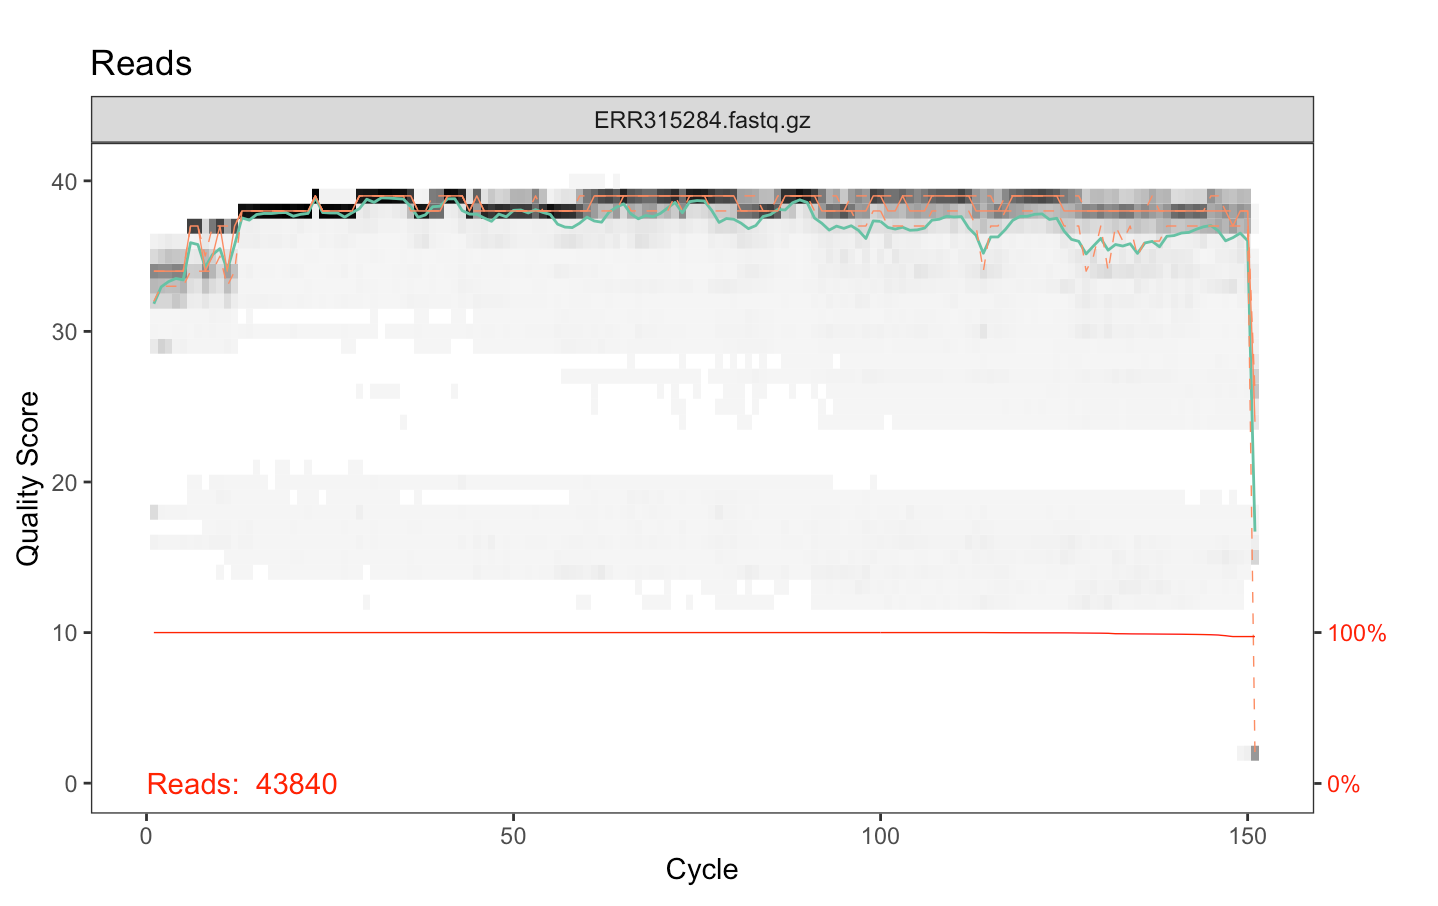
\includegraphics[width=700px]{figure/figure1} \caption{Fastq quality scores for a sample read file}\label{fig:figure1}
\end{figure}
Following the filtration of input reads, we used DADA2 to infer ASVs.
Demultiplexed, dereplicated fastq files were selected for each sample. A
sufficiently large subset of our data was taken, and then the DADA2
iterative sequence inference algorithm was run to estimate error rates.
We inspected the fit between observed error rates and fitted error rates
to verify that our estimations were reasonable (Figure 1.2)
\begin{figure}
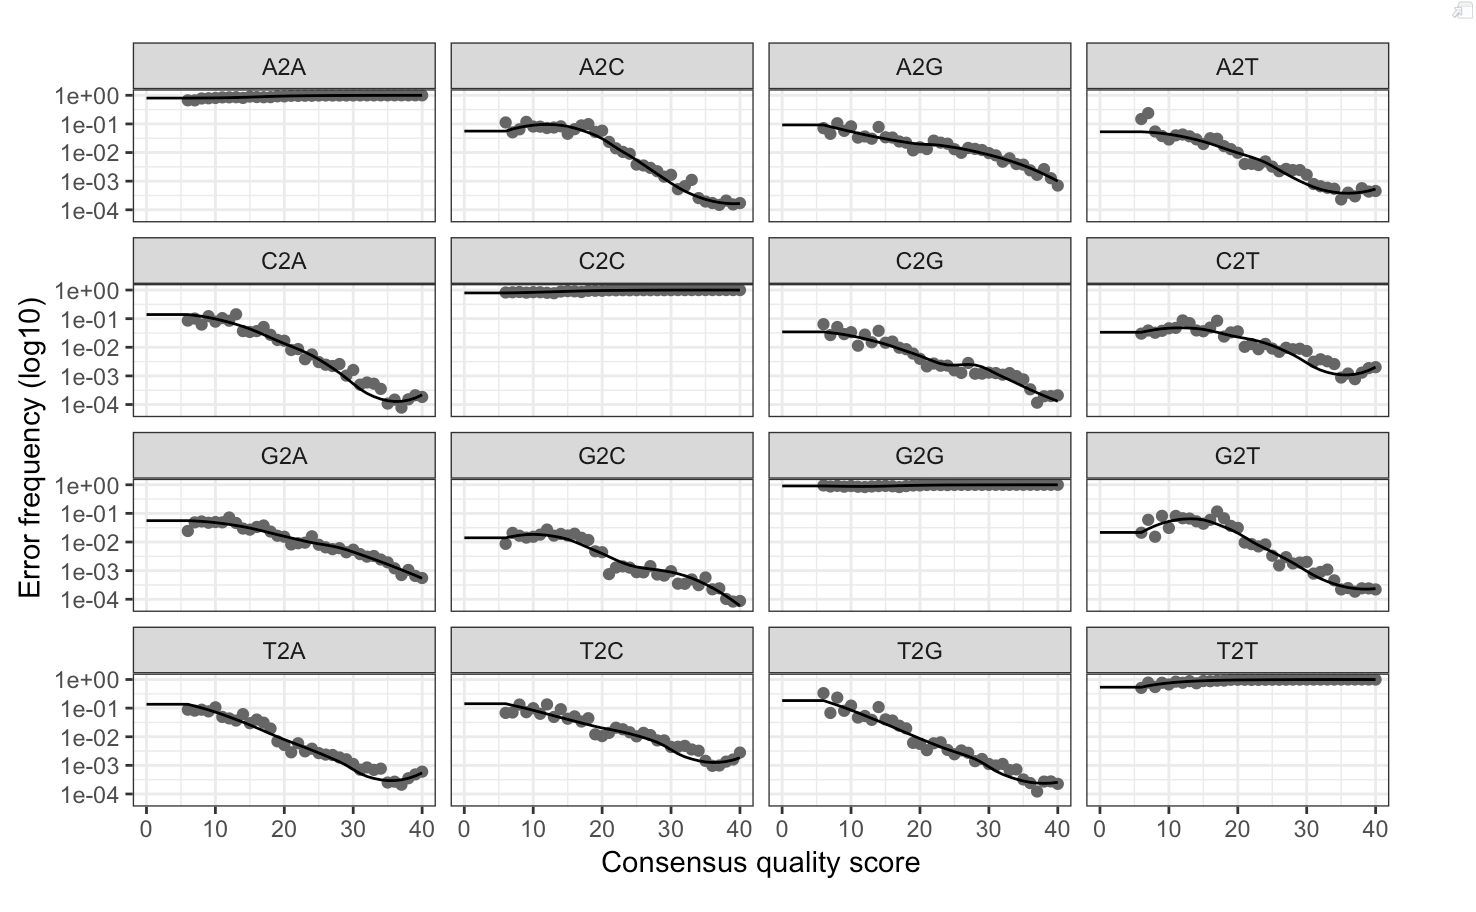
\includegraphics[width=700px]{figure/figure2} \caption{Comparison of observed and fitted error rates from the DADA2 iterative sequence inference algorithm}\label{fig:figure2}
\end{figure}
Using inference on pooled sequencing reads from all samples, DADA2 then
removed nearly all substition and indel errors from our data. Finally, a
sequence table was constructed from our sequences.

Just as processing of sequencing data was completed for the Lozupone
dataset, Alex Sibley, a bioinformatician working with the Sung lab in
the Duke School of Medicine, created an ASV table using the Memorial
Sloan Kettering leukemia data. Given these data, we continued through
the Callahan workflow to further filter and process our data.

\chapter{Post-processing and Filtration of the Sequence
Table}\label{post-processing-and-filtration-of-the-sequence-table}

The ASV table produced by Alex Sibley consisted of seven different
bathces of stool samples produced by MSK. These distinct tables were
merged into a single ASV table, with columns representing different
ASVs, rows representing sampling, and counts in the table representing
the abundance of each ASV in each of our samples.

DADA2 was used to remove chimeric sequences from the sequence table by
comparing each inferred sequence to others in the table, and removing
those that could be reproduced by stitching together two more abundant
sequences. The DADA2 naive Bayesian classifier was then used to compare
sequence variants to the RDP v14 training set of classified sequences
(Cole 2013). Through this process, each ASV column is assigned a full
taxonomy, including Kingdom, Phylum, Class, Order, Family, and Genus.

In addition to assigning taxonomies, we associated deidentified metadata
to our stool samples, also provided to us by Memorial Sloan Kettering.
The metadata were imported, cleaned, and subsetted to match our ASV
table. Finally, the R ``phyloseq'' package was applied to combine our
ASV feature table, our metadata, and our sequence taxonomies of our
amplicon sequencing experiment into a single object (McMurdle 2013).

With our full phyloseq object, we then used our assigned taxonomies as a
filtering criterion on our data. This filtration process helps us to
avoid spending unneeded time on taxa that are seen too infrequently and
eliminates extra noise by deleting taxa that are simply artifacts of
data collection.

We created a table of read counts for each Phylum present in our
dataset.
\begin{longtable}[]{@{}cc@{}}
\caption{Correlation of Inheritance Factors for Parents and
Child}\tabularnewline
\toprule
\begin{minipage}[b]{0.39\columnwidth}\centering\strut
Phyla\strut
\end{minipage} & \begin{minipage}[b]{0.20\columnwidth}\centering\strut
Read Counts\strut
\end{minipage}\tabularnewline
\midrule
\endfirsthead
\toprule
\begin{minipage}[b]{0.39\columnwidth}\centering\strut
Phyla\strut
\end{minipage} & \begin{minipage}[b]{0.20\columnwidth}\centering\strut
Read Counts\strut
\end{minipage}\tabularnewline
\midrule
\endhead
\begin{minipage}[t]{0.39\columnwidth}\centering\strut
Actinobacteria\strut
\end{minipage} & \begin{minipage}[t]{0.20\columnwidth}\centering\strut
3864\strut
\end{minipage}\tabularnewline
\begin{minipage}[t]{0.39\columnwidth}\centering\strut
Armatimonadetes\strut
\end{minipage} & \begin{minipage}[t]{0.20\columnwidth}\centering\strut
1\strut
\end{minipage}\tabularnewline
\begin{minipage}[t]{0.39\columnwidth}\centering\strut
Bacteroidetes\strut
\end{minipage} & \begin{minipage}[t]{0.20\columnwidth}\centering\strut
3375\strut
\end{minipage}\tabularnewline
\begin{minipage}[t]{0.39\columnwidth}\centering\strut
Chlamydiae\strut
\end{minipage} & \begin{minipage}[t]{0.20\columnwidth}\centering\strut
3\strut
\end{minipage}\tabularnewline
\begin{minipage}[t]{0.39\columnwidth}\centering\strut
Cyanobacteria/Chloroplast\strut
\end{minipage} & \begin{minipage}[t]{0.20\columnwidth}\centering\strut
15\strut
\end{minipage}\tabularnewline
\begin{minipage}[t]{0.39\columnwidth}\centering\strut
Deferribacteres\strut
\end{minipage} & \begin{minipage}[t]{0.20\columnwidth}\centering\strut
1\strut
\end{minipage}\tabularnewline
\begin{minipage}[t]{0.39\columnwidth}\centering\strut
Deinococcus-Thermus\strut
\end{minipage} & \begin{minipage}[t]{0.20\columnwidth}\centering\strut
3\strut
\end{minipage}\tabularnewline
\begin{minipage}[t]{0.39\columnwidth}\centering\strut
Euryarchaeota\strut
\end{minipage} & \begin{minipage}[t]{0.20\columnwidth}\centering\strut
2\strut
\end{minipage}\tabularnewline
\begin{minipage}[t]{0.39\columnwidth}\centering\strut
Firmicutes\strut
\end{minipage} & \begin{minipage}[t]{0.20\columnwidth}\centering\strut
155578\strut
\end{minipage}\tabularnewline
\begin{minipage}[t]{0.39\columnwidth}\centering\strut
Fusobacteria\strut
\end{minipage} & \begin{minipage}[t]{0.20\columnwidth}\centering\strut
19\strut
\end{minipage}\tabularnewline
\begin{minipage}[t]{0.39\columnwidth}\centering\strut
Proteobacteria\strut
\end{minipage} & \begin{minipage}[t]{0.20\columnwidth}\centering\strut
3481\strut
\end{minipage}\tabularnewline
\begin{minipage}[t]{0.39\columnwidth}\centering\strut
Spirochaetes\strut
\end{minipage} & \begin{minipage}[t]{0.20\columnwidth}\centering\strut
4\strut
\end{minipage}\tabularnewline
\begin{minipage}[t]{0.39\columnwidth}\centering\strut
Synergistetes\strut
\end{minipage} & \begin{minipage}[t]{0.20\columnwidth}\centering\strut
84\strut
\end{minipage}\tabularnewline
\begin{minipage}[t]{0.39\columnwidth}\centering\strut
Tenericutes\strut
\end{minipage} & \begin{minipage}[t]{0.20\columnwidth}\centering\strut
3\strut
\end{minipage}\tabularnewline
\begin{minipage}[t]{0.39\columnwidth}\centering\strut
Verrumicrobia\strut
\end{minipage} & \begin{minipage}[t]{0.20\columnwidth}\centering\strut
8823\strut
\end{minipage}\tabularnewline
\begin{minipage}[t]{0.39\columnwidth}\centering\strut
Woesearchaeota\strut
\end{minipage} & \begin{minipage}[t]{0.20\columnwidth}\centering\strut
1578\strut
\end{minipage}\tabularnewline
\begin{minipage}[t]{0.39\columnwidth}\centering\strut
\strut
\end{minipage} & \begin{minipage}[t]{0.20\columnwidth}\centering\strut
211134\strut
\end{minipage}\tabularnewline
\bottomrule
\end{longtable}
Many of our features are annotated with a phylum of ``NA,'' potentially
indicating that they are artifacts. However, due to the fact that
databases such as the RDP are often far from complete, filtering out all
of these datapoints was considered to be too stringent. As a result,
they were kept in our dataset.

We also explored feature prevalence in our dataset. Feature prevalence
is defined to be the number of samples in which a taxum appears at least
once. We computed the average and total prevalences of the features in
each phylum to determine if there were any phyla that consisted mostly
of low-prevalence features.
\begin{longtable}[]{@{}ccc@{}}
\caption{Feature Prevalence of Phyla in our Dataset}\tabularnewline
\toprule
\begin{minipage}[b]{0.35\columnwidth}\centering\strut
Phylum\strut
\end{minipage} & \begin{minipage}[b]{0.28\columnwidth}\centering\strut
Average Abundance\strut
\end{minipage} & \begin{minipage}[b]{0.28\columnwidth}\centering\strut
Total Abundance\strut
\end{minipage}\tabularnewline
\midrule
\endfirsthead
\toprule
\begin{minipage}[b]{0.35\columnwidth}\centering\strut
Phylum\strut
\end{minipage} & \begin{minipage}[b]{0.28\columnwidth}\centering\strut
Average Abundance\strut
\end{minipage} & \begin{minipage}[b]{0.28\columnwidth}\centering\strut
Total Abundance\strut
\end{minipage}\tabularnewline
\midrule
\endhead
\begin{minipage}[t]{0.35\columnwidth}\centering\strut
Actinobacteria\strut
\end{minipage} & \begin{minipage}[t]{0.28\columnwidth}\centering\strut
2.612319\strut
\end{minipage} & \begin{minipage}[t]{0.28\columnwidth}\centering\strut
10094\strut
\end{minipage}\tabularnewline
\begin{minipage}[t]{0.35\columnwidth}\centering\strut
Armatimonadetes\strut
\end{minipage} & \begin{minipage}[t]{0.28\columnwidth}\centering\strut
1.000000\strut
\end{minipage} & \begin{minipage}[t]{0.28\columnwidth}\centering\strut
1\strut
\end{minipage}\tabularnewline
\begin{minipage}[t]{0.35\columnwidth}\centering\strut
Bacteroidetes\strut
\end{minipage} & \begin{minipage}[t]{0.28\columnwidth}\centering\strut
3.135111\strut
\end{minipage} & \begin{minipage}[t]{0.28\columnwidth}\centering\strut
10581\strut
\end{minipage}\tabularnewline
\begin{minipage}[t]{0.35\columnwidth}\centering\strut
Chlamydiae\strut
\end{minipage} & \begin{minipage}[t]{0.28\columnwidth}\centering\strut
1.000000\strut
\end{minipage} & \begin{minipage}[t]{0.28\columnwidth}\centering\strut
3\strut
\end{minipage}\tabularnewline
\begin{minipage}[t]{0.35\columnwidth}\centering\strut
Cyanobacteria/Chloroplast\strut
\end{minipage} & \begin{minipage}[t]{0.28\columnwidth}\centering\strut
3.133333\strut
\end{minipage} & \begin{minipage}[t]{0.28\columnwidth}\centering\strut
47\strut
\end{minipage}\tabularnewline
\begin{minipage}[t]{0.35\columnwidth}\centering\strut
Deferribacteres\strut
\end{minipage} & \begin{minipage}[t]{0.28\columnwidth}\centering\strut
7.000000\strut
\end{minipage} & \begin{minipage}[t]{0.28\columnwidth}\centering\strut
7\strut
\end{minipage}\tabularnewline
\begin{minipage}[t]{0.35\columnwidth}\centering\strut
Deinococcus-Thermus\strut
\end{minipage} & \begin{minipage}[t]{0.28\columnwidth}\centering\strut
2.333333\strut
\end{minipage} & \begin{minipage}[t]{0.28\columnwidth}\centering\strut
7\strut
\end{minipage}\tabularnewline
\begin{minipage}[t]{0.35\columnwidth}\centering\strut
Euryarchaeota\strut
\end{minipage} & \begin{minipage}[t]{0.28\columnwidth}\centering\strut
25.000000\strut
\end{minipage} & \begin{minipage}[t]{0.28\columnwidth}\centering\strut
50\strut
\end{minipage}\tabularnewline
\begin{minipage}[t]{0.35\columnwidth}\centering\strut
Firmicutes\strut
\end{minipage} & \begin{minipage}[t]{0.28\columnwidth}\centering\strut
1.952770\strut
\end{minipage} & \begin{minipage}[t]{0.28\columnwidth}\centering\strut
303808\strut
\end{minipage}\tabularnewline
\begin{minipage}[t]{0.35\columnwidth}\centering\strut
Fusobacteria\strut
\end{minipage} & \begin{minipage}[t]{0.28\columnwidth}\centering\strut
4.473684\strut
\end{minipage} & \begin{minipage}[t]{0.28\columnwidth}\centering\strut
85\strut
\end{minipage}\tabularnewline
\begin{minipage}[t]{0.35\columnwidth}\centering\strut
Proteobacteria\strut
\end{minipage} & \begin{minipage}[t]{0.28\columnwidth}\centering\strut
3.381212\strut
\end{minipage} & \begin{minipage}[t]{0.28\columnwidth}\centering\strut
11770\strut
\end{minipage}\tabularnewline
\begin{minipage}[t]{0.35\columnwidth}\centering\strut
Spirochaetes\strut
\end{minipage} & \begin{minipage}[t]{0.28\columnwidth}\centering\strut
1.500000\strut
\end{minipage} & \begin{minipage}[t]{0.28\columnwidth}\centering\strut
6\strut
\end{minipage}\tabularnewline
\begin{minipage}[t]{0.35\columnwidth}\centering\strut
Synergistetes\strut
\end{minipage} & \begin{minipage}[t]{0.28\columnwidth}\centering\strut
1.880952\strut
\end{minipage} & \begin{minipage}[t]{0.28\columnwidth}\centering\strut
158\strut
\end{minipage}\tabularnewline
\begin{minipage}[t]{0.35\columnwidth}\centering\strut
Tenericutes\strut
\end{minipage} & \begin{minipage}[t]{0.28\columnwidth}\centering\strut
2.333333\strut
\end{minipage} & \begin{minipage}[t]{0.28\columnwidth}\centering\strut
7\strut
\end{minipage}\tabularnewline
\begin{minipage}[t]{0.35\columnwidth}\centering\strut
Verrucomicrobia\strut
\end{minipage} & \begin{minipage}[t]{0.28\columnwidth}\centering\strut
1.706562\strut
\end{minipage} & \begin{minipage}[t]{0.28\columnwidth}\centering\strut
15057\strut
\end{minipage}\tabularnewline
\begin{minipage}[t]{0.35\columnwidth}\centering\strut
Woesearchaeota\strut
\end{minipage} & \begin{minipage}[t]{0.28\columnwidth}\centering\strut
3.147022\strut
\end{minipage} & \begin{minipage}[t]{0.28\columnwidth}\centering\strut
4966\strut
\end{minipage}\tabularnewline
\begin{minipage}[t]{0.35\columnwidth}\centering\strut
\strut
\end{minipage} & \begin{minipage}[t]{0.28\columnwidth}\centering\strut
1.977450\strut
\end{minipage} & \begin{minipage}[t]{0.28\columnwidth}\centering\strut
417507\strut
\end{minipage}\tabularnewline
\bottomrule
\end{longtable}
Through this process, we dropped the following phyla from our dataset:
Armatimonadetes, Chlamydiae, Deferribacteres, Deinococcus-Thermus,
Spirochaetes, and Tenericutes

The previous filtration steps required our taxonomic annotations to
properly work. Without taxonomies, we can use prevalence filtering as a
form of unsupervised filtration to further streamline our data. We
plotted graphs of prevalence against total abundance for each phylum in
an effort to identify an appropriate prevalence threshold (Figure 2.1).
\begin{figure}
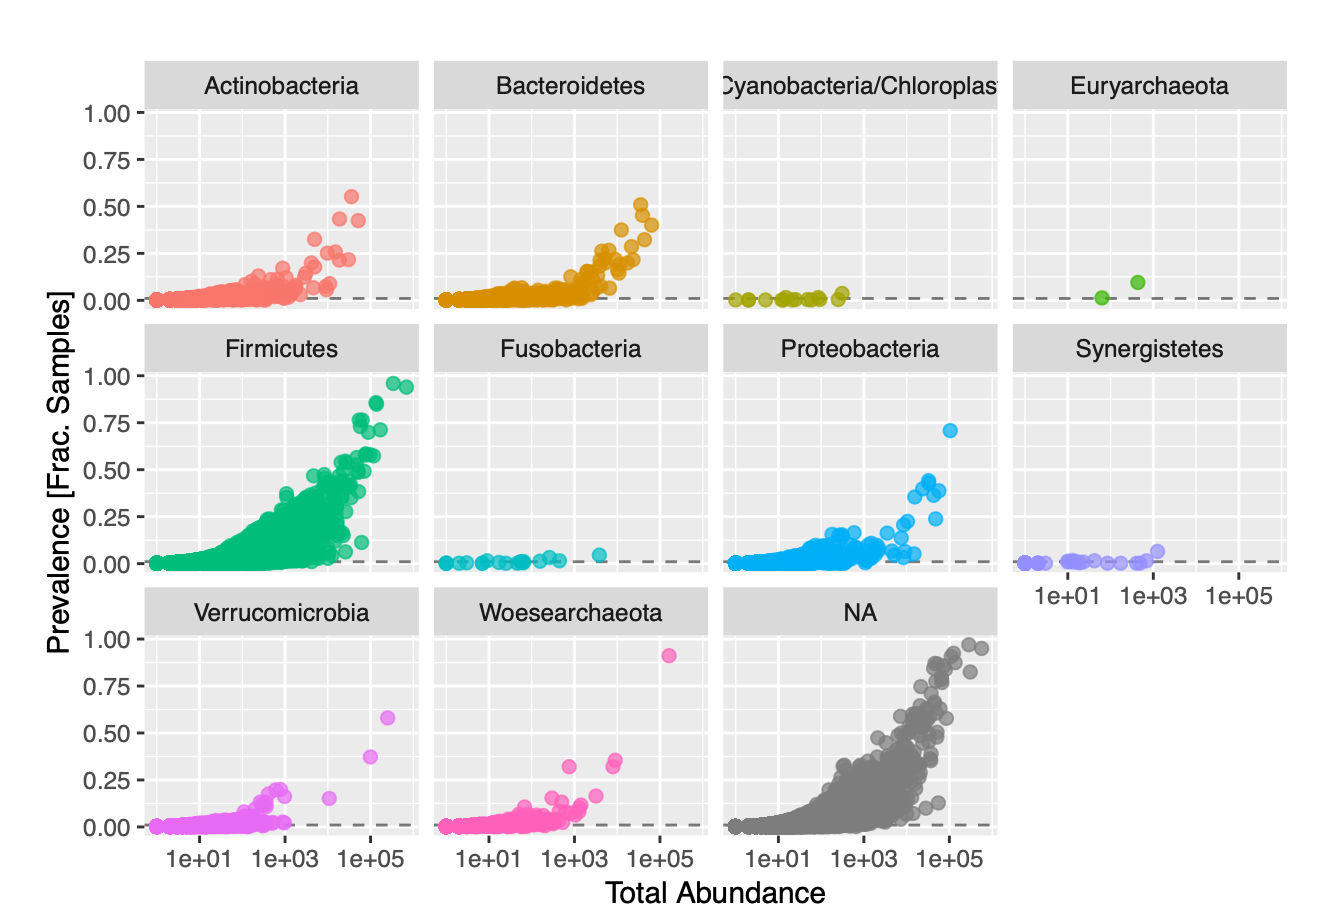
\includegraphics[width=700px]{figure/figure3} \caption{Feature Prevalence of Phyla against Total Abundance in our Dataset}\label{fig:figure3}
\end{figure}
We failed to see see any real separation in our plots, so we established
an arbitrary prevalence threshold of 1\%.

In order to account for differences in library size, variance, and
scale, we had to use relative abundances instead of total abundances. We
transformed our data from counts to frequencies, and also applied a log
transformation. We then applied Principal Coordinates Analysis (PCoA)
with Bray-Curtis dissimilarity to our transformed data.

We visualized ordination plots of the samples in our dataset, as well as
of the distribution of taxa present in each sample (Figure 2.2).
\begin{figure}
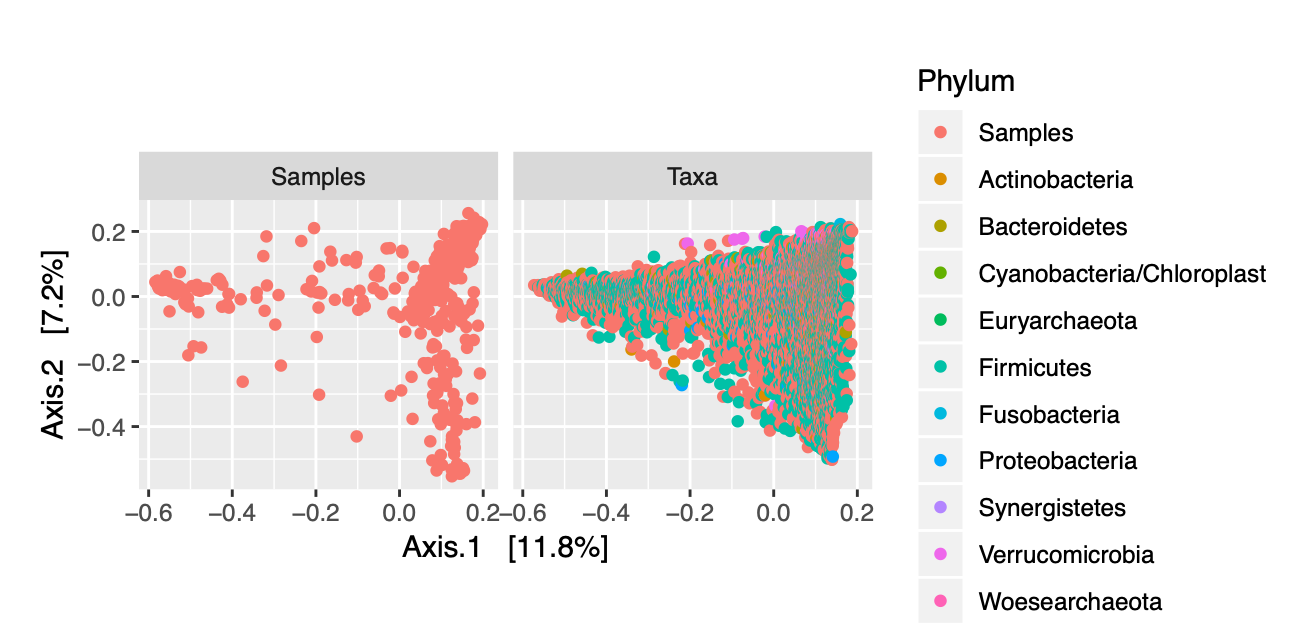
\includegraphics[width=700px]{figure/figure4} \caption{Ordination Plots of Samples and of Phyla}\label{fig:figure4}
\end{figure}
In addition to looking at the specific distribution of phyla for our
samples, we can color-code the different datapoints representing each of
our samples to determine if there are any obvious clustering patterns
based upon the covariates in our metadata. In the following two plots,
we visualize vital status and graft source for our patients across all
time points (Figures 2.3 and 2.4).
\begin{figure}
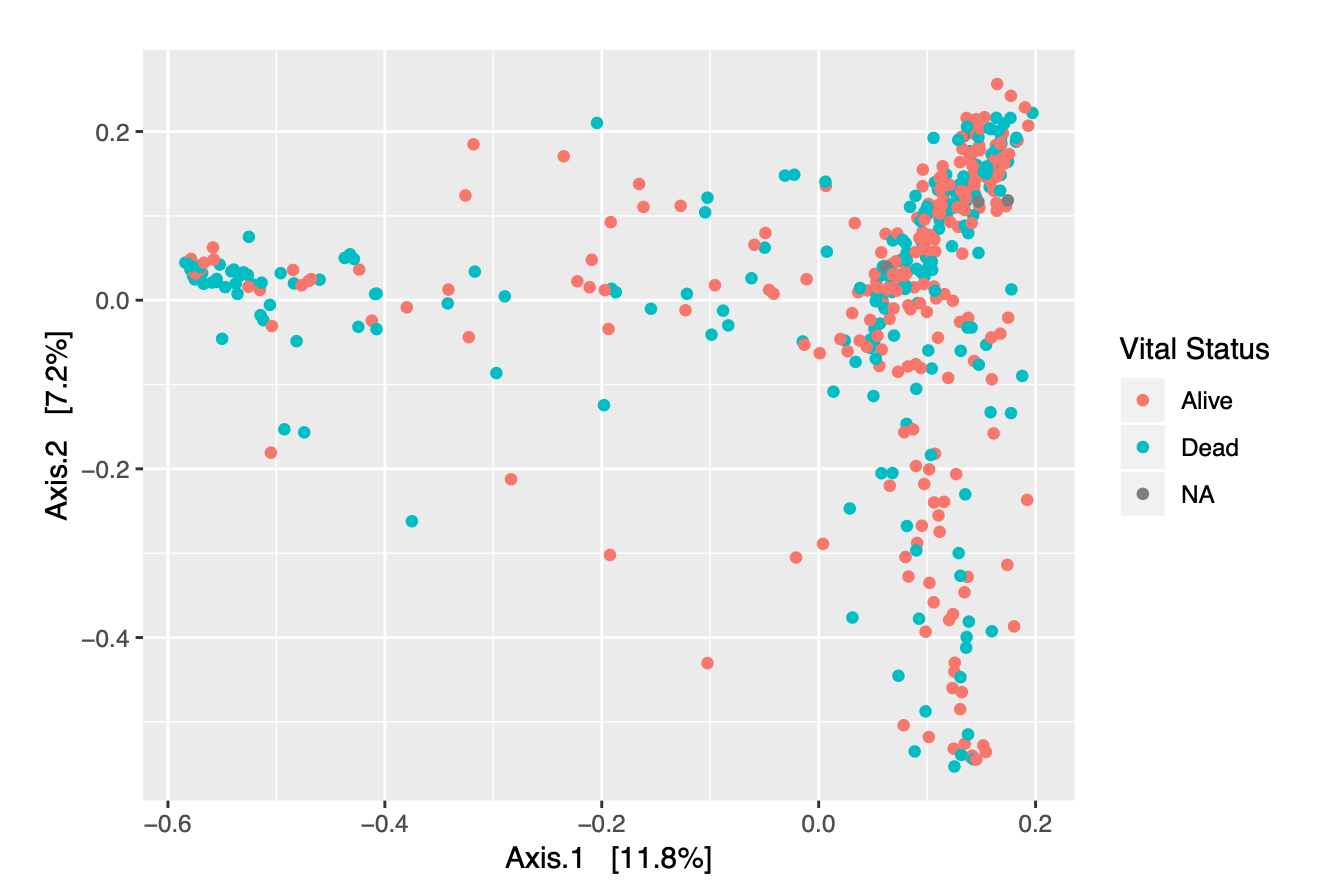
\includegraphics[width=700px]{figure/figure5} \caption{Ordination Plot of Samples, colored by Vital Status}\label{fig:figure5}
\end{figure}
\begin{figure}
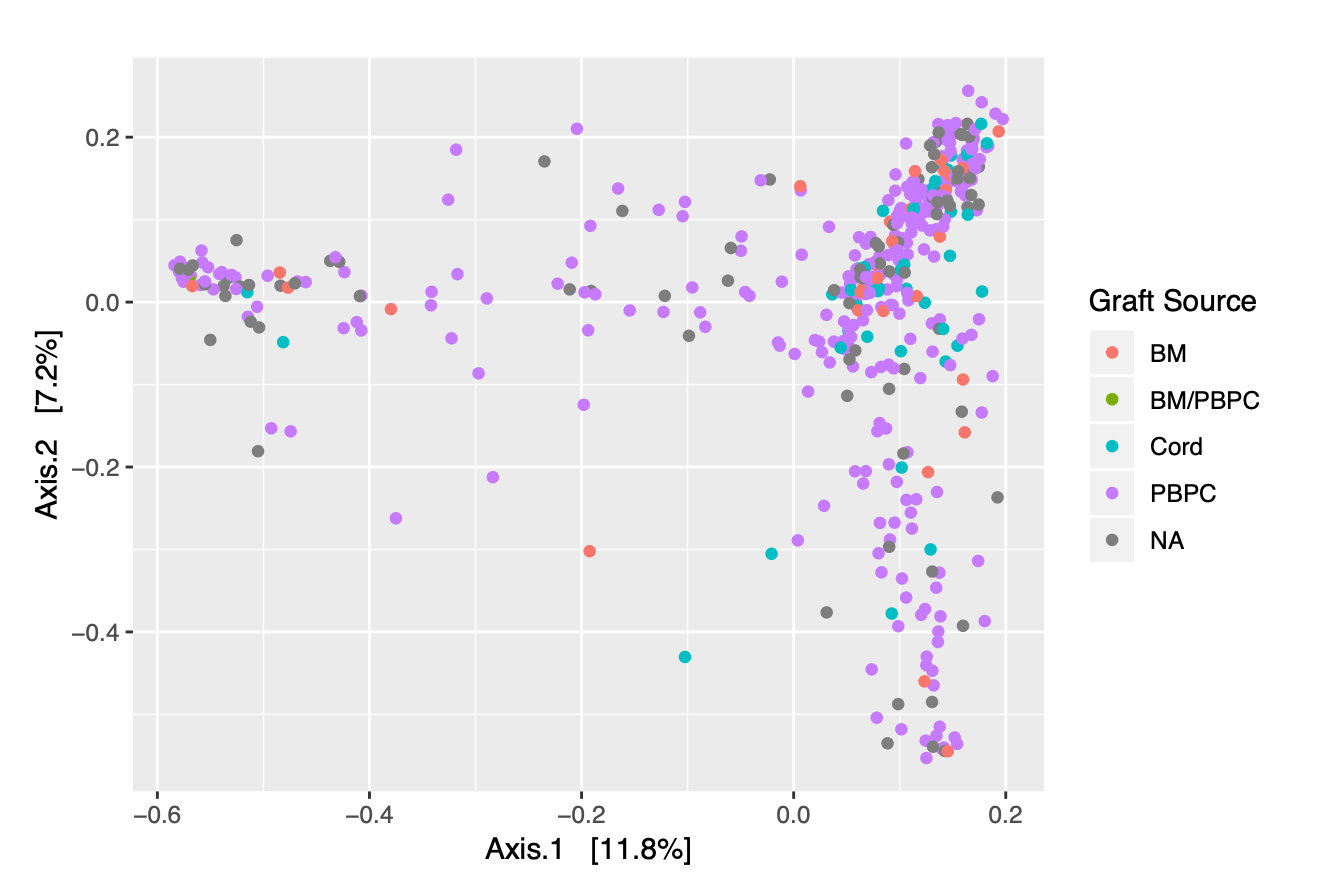
\includegraphics[width=700px]{figure/figure6} \caption{Ordination Plot of Samples, colored by Graft Source}\label{fig:figure6}
\end{figure}
While these visualizations revealed some information into the
distributions of bacteria in our samples, we failed to see any obvious
trends across our categories. Another key issue with our plots is that
we were unable to clearly identify how a single patient's sample would
change over time. To quantify the dynamics of a patient's microbiome in
our ordination plot, we devised two different summary statistics:
maximum distance and last distance.

We began by creating a Scree plot to determine the contributions of our
different principal coordinate axes (Figure 2.5).
\begin{figure}
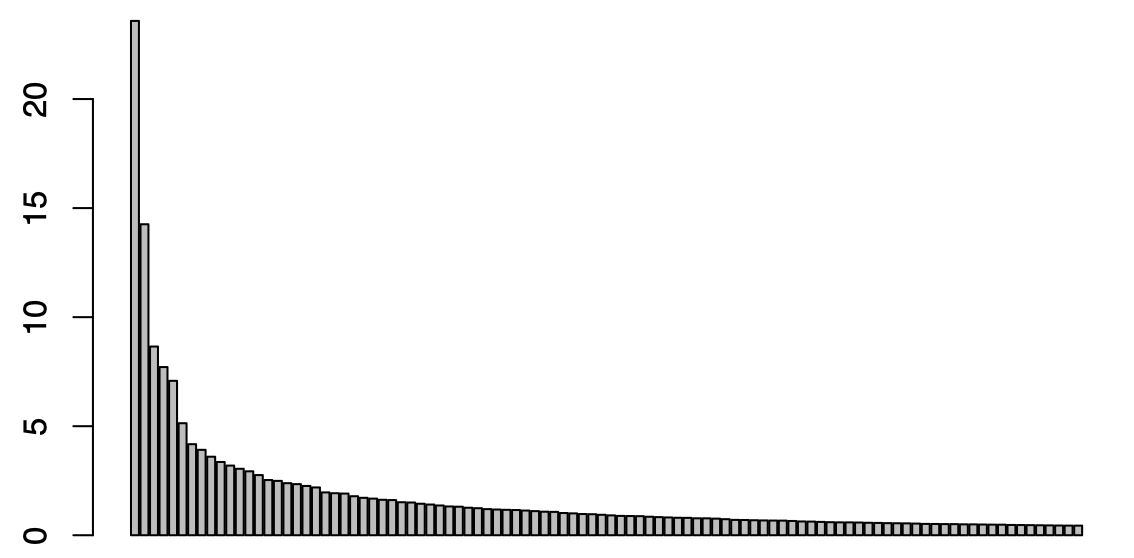
\includegraphics[width=700px]{figure/figure7} \caption{Scree Plot of Contributions from PCoA Axes}\label{fig:figure7}
\end{figure}
Analyzing the plot and computing the contributions of our axes, we see
that the first 17 axes constitute the the majority of contributions from
our 460 total axes. So, we used these axes as part of our distance
metrics; we calculated the distance from one sample to another by taking
the square root of the sum of the squared differences of each of our
seventeen components.

Given an individual patient in our dataset, maximum distance is defined
as the furthest distance in the ordination plot traveled from the
patient's earliest point. Last distance is defined as the distance
between the individual's earliest and latest point in the ordination
plot. A potential future avenue to explore in this scenario is to scale
principal components relative to one another instead of simply using the
first seventeen, in an effort to get a better quantification of our two
metrics. With our processed dataset and ordination plot, and our new
summary statistics, we turned to the visualization application
``Tableau.''

\chapter{Interactive Visualizations in
Tableau}\label{interactive-visualizations-in-tableau}

Tableau is a user-friendly application helpful in the design of
interactive visualizations. We used this application to visualize the
our data over time in our ordination plots and determine if there were
any noticeable associations between variables in our metadata and the
dynamics of our samples.

In each Tableau sheet created, hovering over a single point will cause
that sample, as well as all other samples corresponding to the same
patient, to be highlighted. This behavior allows us to specifically
visualize how our samples' distributions change on an individual basis.

Figures 3.1, 3.2, and 3.3 include some examples of the plots designed in
Tableau.

Figure 3.1 depicts an ordination plot, colored by Batch number, and
connected by patient ID. The thickness of lines connecting points to one
another increases as time progresses. Hovering over a point will also
highlight other sample points and the path representative of the
selected patient.
\begin{figure}
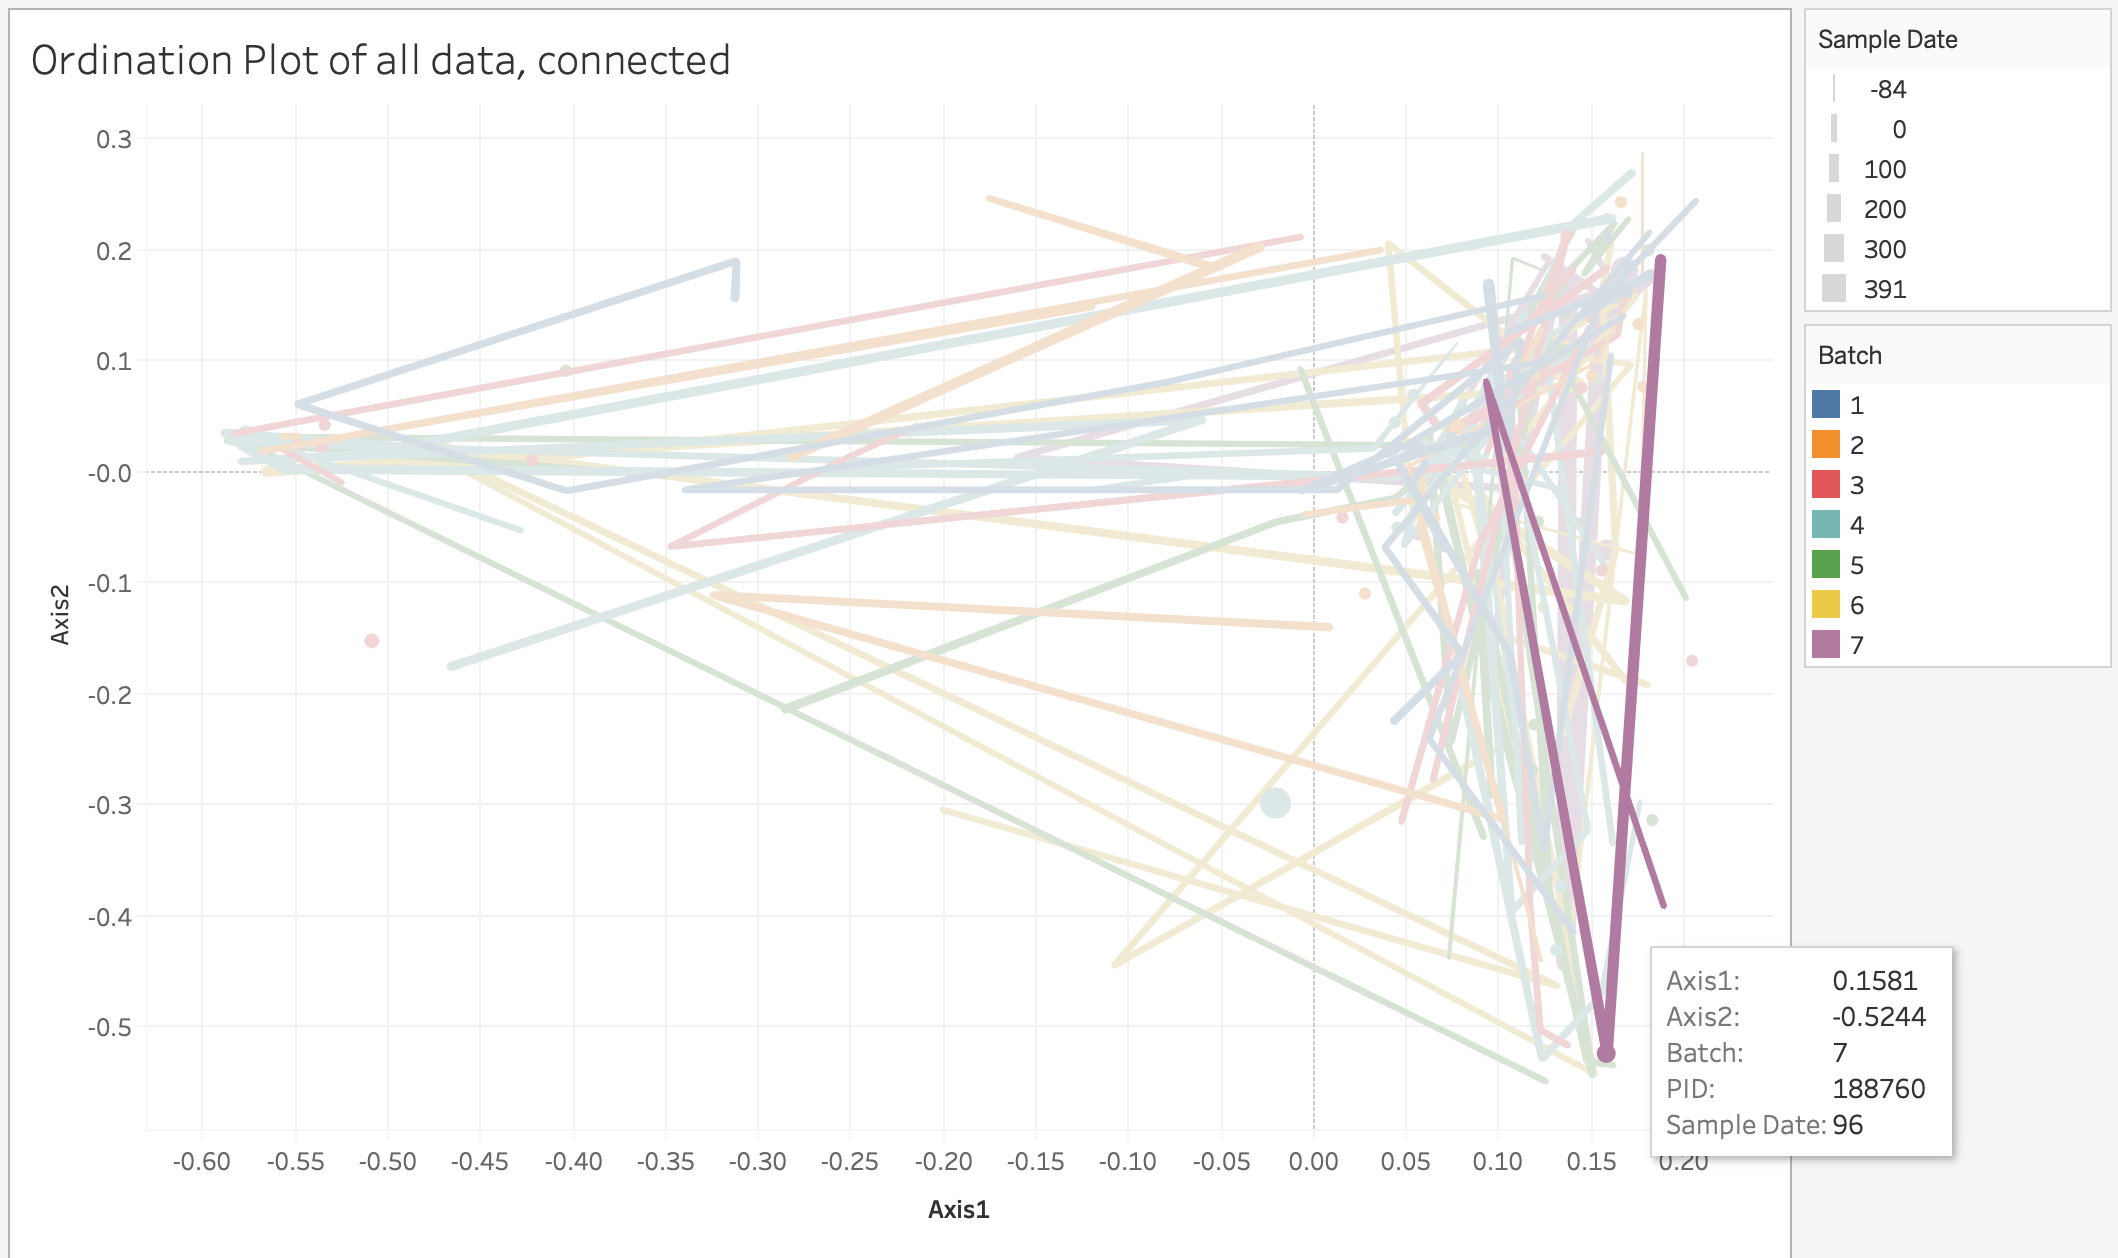
\includegraphics[width=700px]{figure/figure8} \caption{Ordination Plot colored by Batch Number and connected by Patient ID}\label{fig:figure8}
\end{figure}
Figure 3.2 shows plots of the maximum distance travelled by different
patients, separated by whether or not their first sample date occurred
before or after their transplant. It appears roughly that patients with
first time points occurring before transplant date may have potentially
higher maximum distances.
\begin{figure}
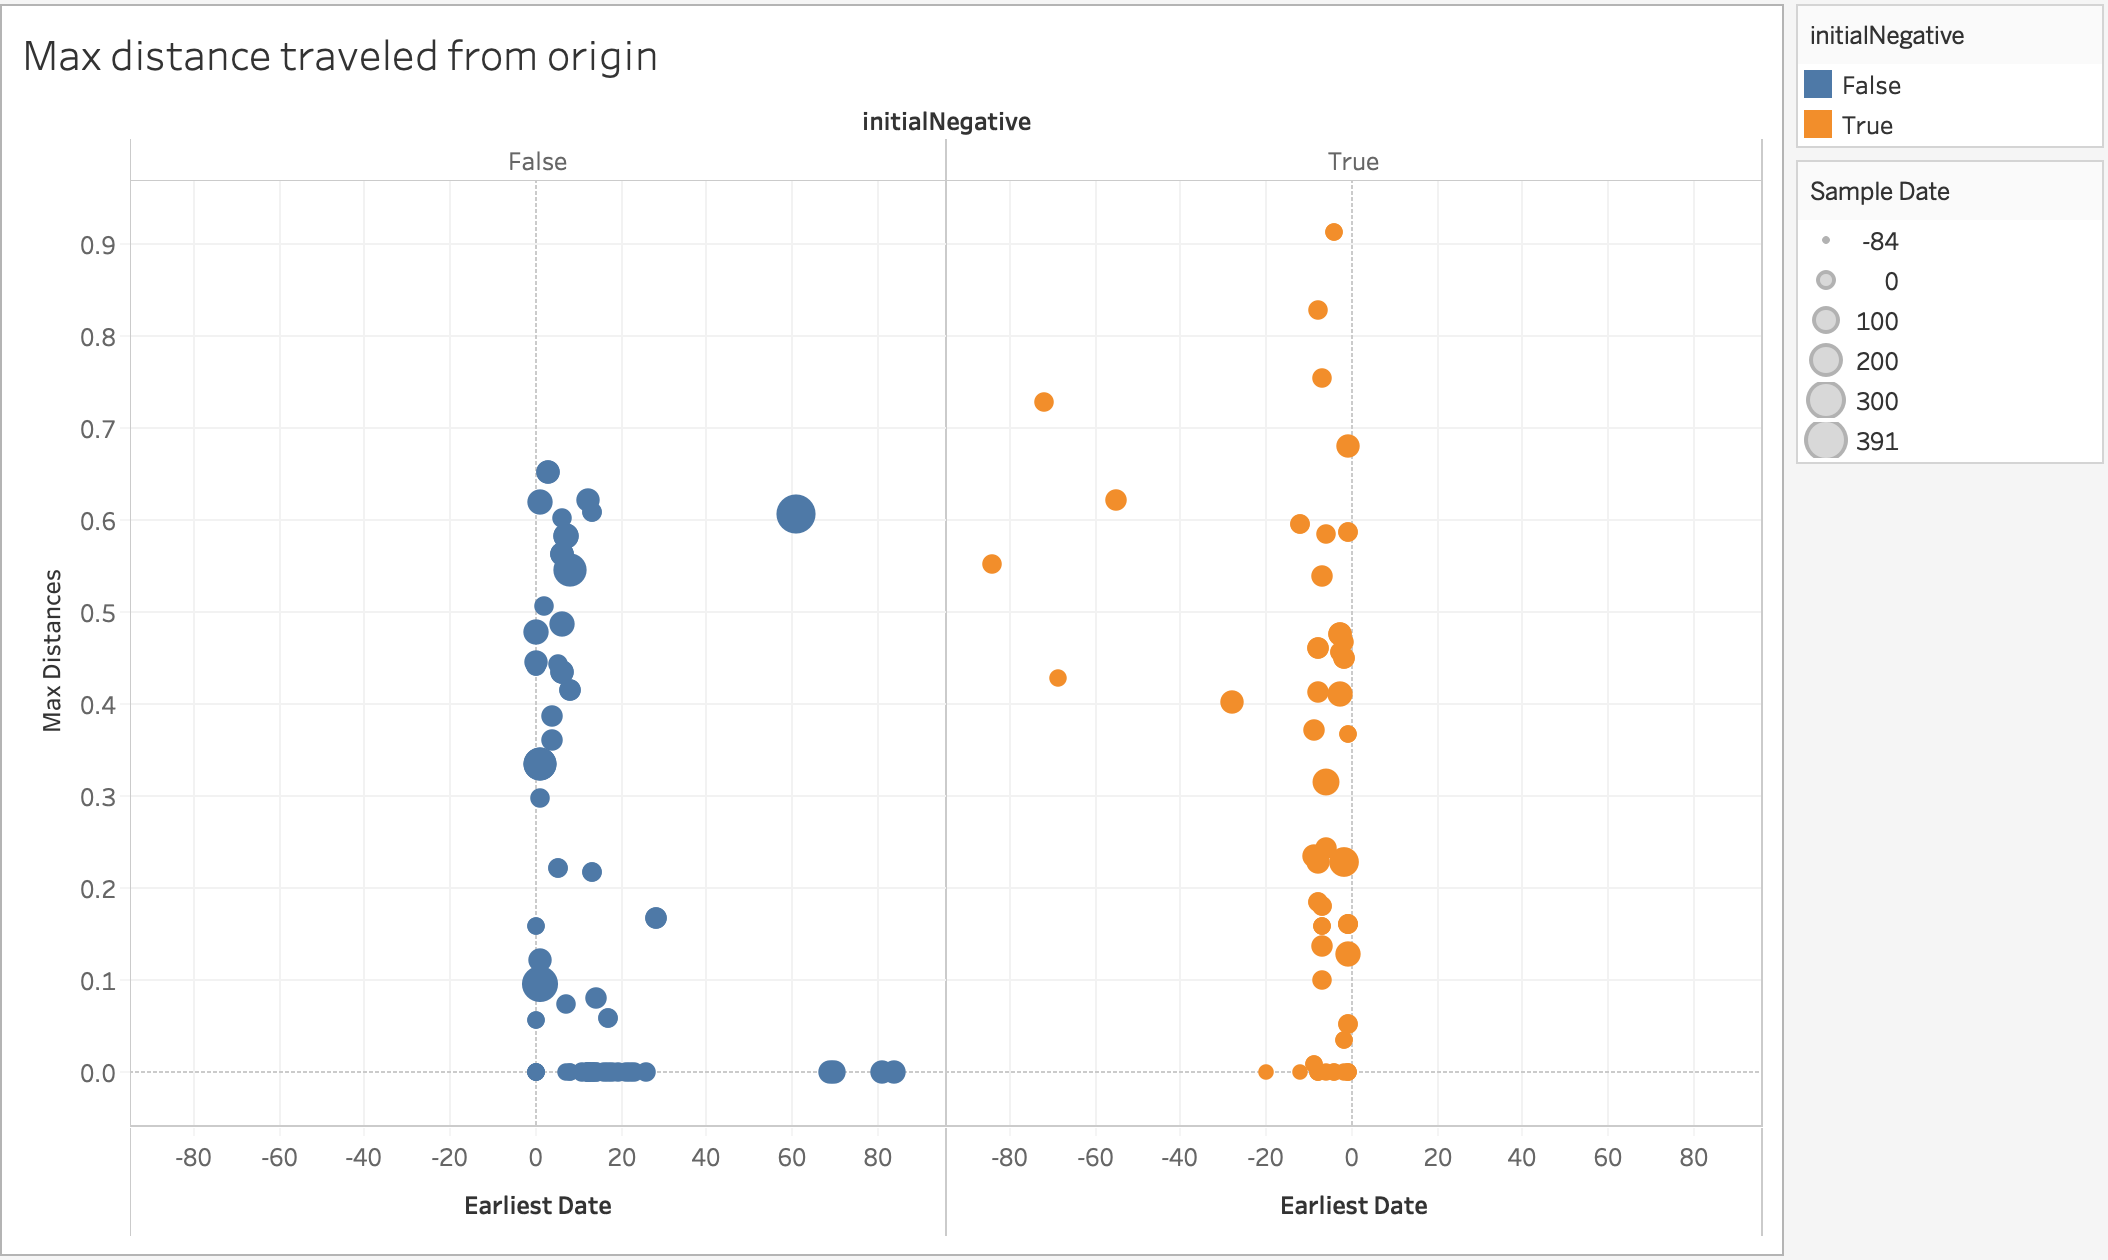
\includegraphics[width=700px]{figure/figure9} \caption{Plots of Maximum Distance traveled by Patient Microbiome}\label{fig:figure9}
\end{figure}
Figure 3.3 depicts two ordination plots colored by presence of acute
graft versus host disease. The top plot depicts agvhd values taken
within the twelve weeks prior to transplants, and the second plot
depicts agvhd values taken within the twelve weeks after. Both plots can
be manipulated to specify the desired time frame. This kind of
visualization allows us to more directly compare the distributions of
our covariates at different times.
\begin{figure}
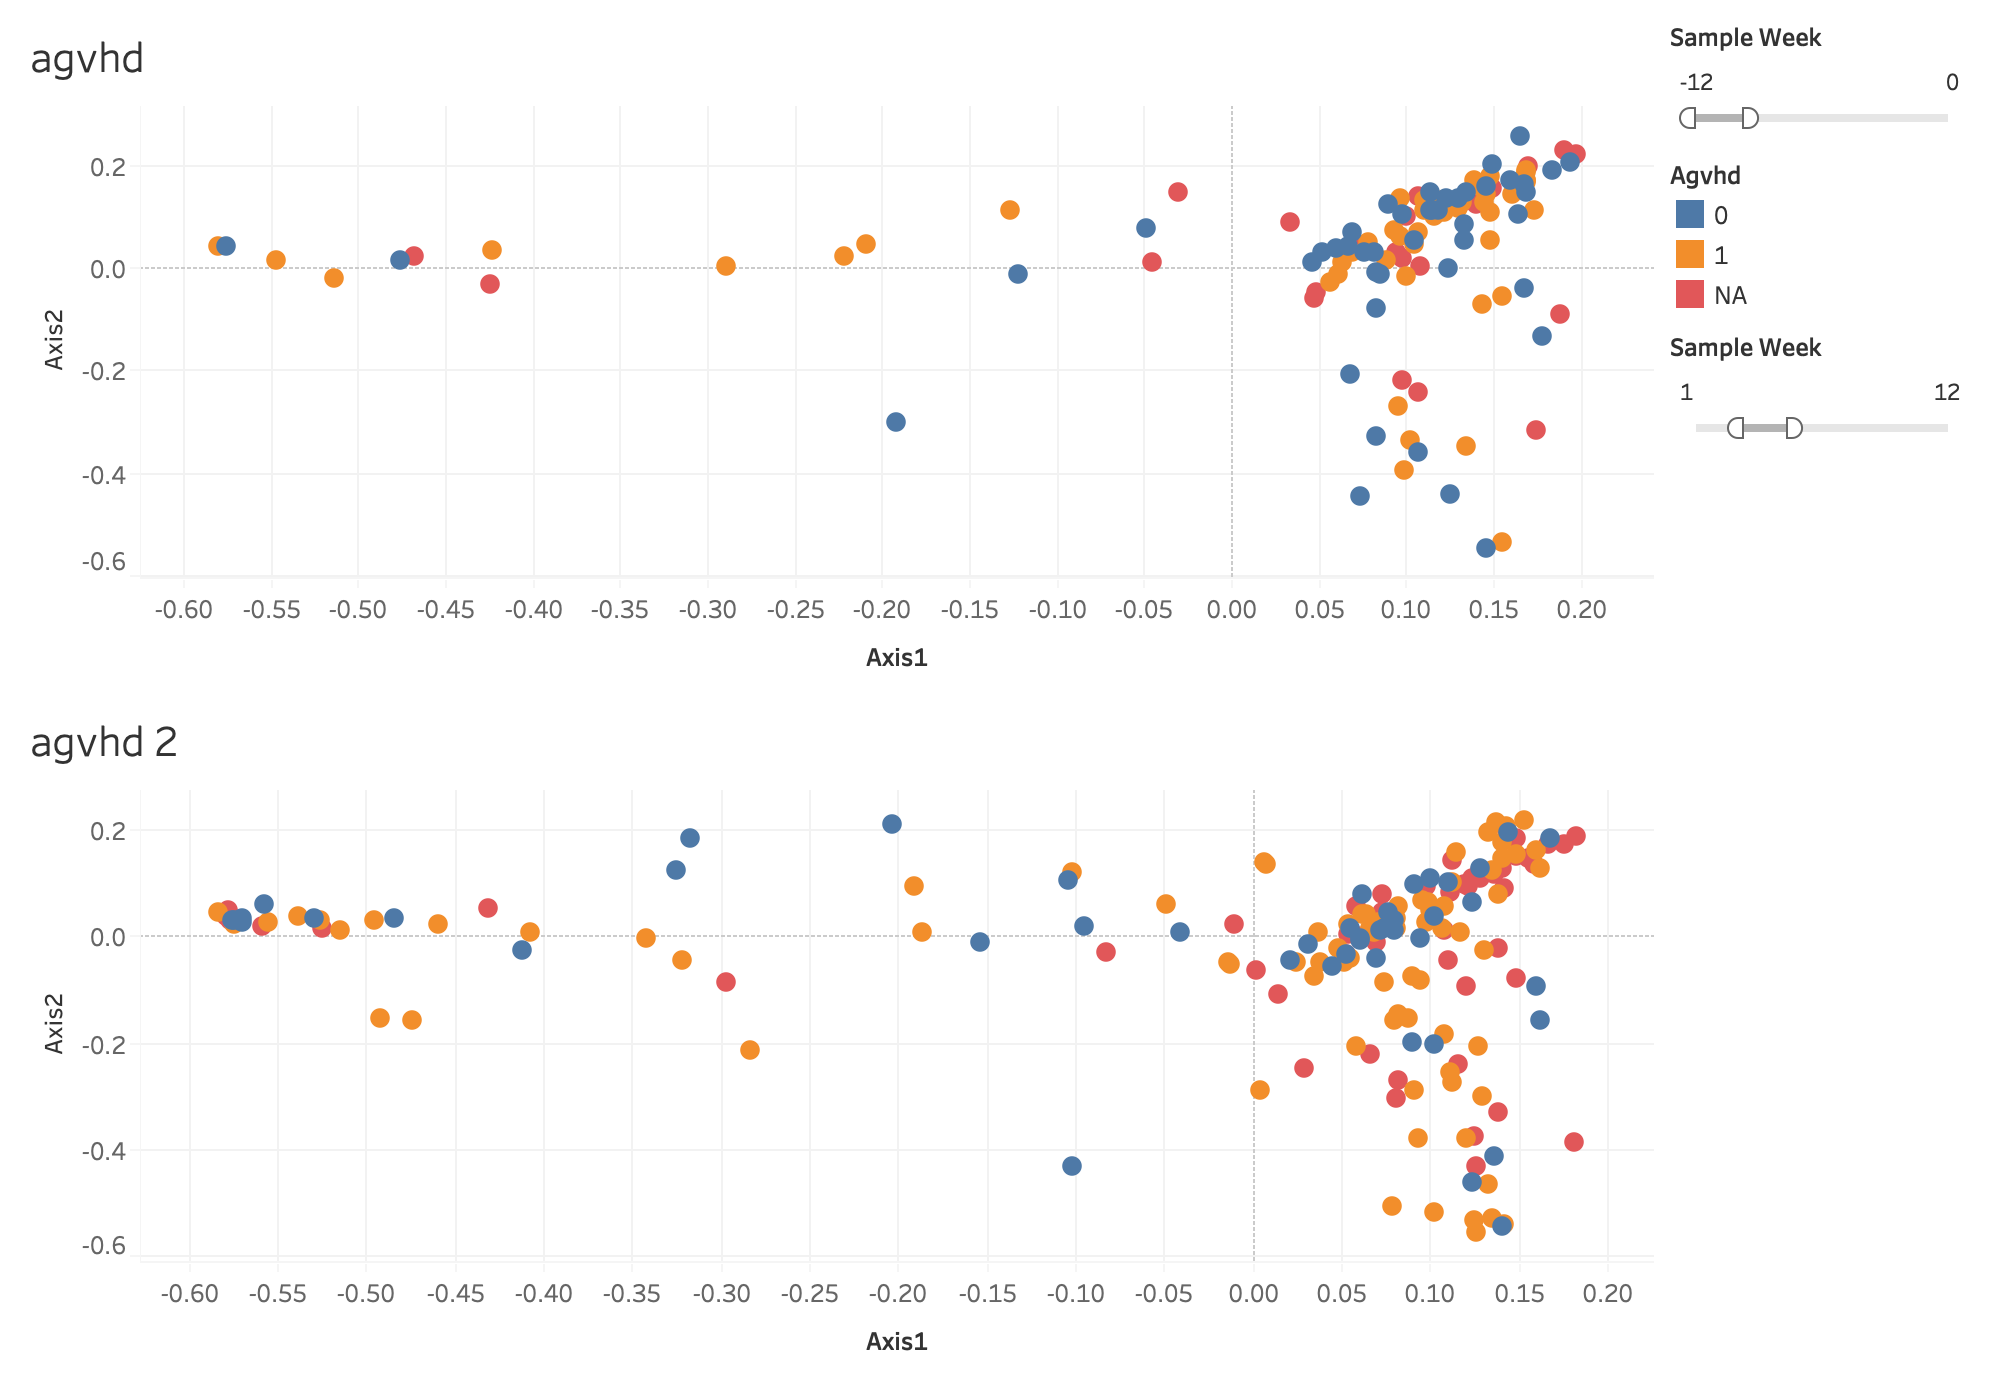
\includegraphics[width=700px]{figure/figure10} \caption{Ordination Plots colored by AGVHD, separated by Time}\label{fig:figure10}
\end{figure}
With all of these plots, we were better able to interact with our data
and the metrics that we had devised. However, while these visualizations
were informative, we were still unable to specifically quantify
potential associations between our various covariates and the dynamics
of the gut microbiome.

\chapter{Linear Regression on Summary
Statistics}\label{linear-regression-on-summary-statistics}

With the processing and filtration of our data, as well as its
visualization in Tableau, we turned to basic linear regressions as well
as non-parametric statistical tests to attempt to evaluate how our
covariates may be linked to the dynamics of the microbiome.

Based upon exploratory data analysis, we kept all of our continuous
variables untransformed. There were no extremely concerning trends in
any of our categorical variables either, so we did not transform them.
There was also no need to transform the outcome variable of maximum
distance.

We used lattice plots to search for interaction effects across our
categorical variables, as well as boxplots to search for connections
between categorical and quantitatie covariates. Identified interactions
were included in our baseline model. Backwards selection was then
performed using AIC as a scoring criterion.

For maximum distance as the outcome, our final model with the lowest AIC
based on backward selection came out to be as follows:

\(maxDistance_{i} = {\beta_{transplantAge}}transplantAge_{i} + {\beta_{AlloDLI}}I(transplantType_{i}=AlloDLI) + {\beta_{Auto}}I(transplantType_{i}=Auto) +{\beta_{Cord}}I(graftSource_{i}=Cord) + {\beta_{PBPC}}I(graftSource_{i}=PBPC) + {\beta_{Dead}}I(vitalStatus_{i}=Dead) + {\beta_{CGVHD}}I(CGVHD_{i}=1)+ {\beta_{anc500}}anc500_{i} + {\beta_{careEnv2}}I(careEnv_{i}=2) + {\beta_{careEnv3}}I(careEnv_{i}=3) + {\beta_{totalTimeSpan}}totalTimeSpan_{i} + {\beta_{vitalStatus/careEnv2}}I(vitalStatus/careEnv2_{i}=1) + {\beta_{vitalStatus/careEnv3}}I(vitalStatus/careEnv3_{i}=1)\)

This model had an AIC of -34.11267, and it identified the following
covariates as significant:
\begin{longtable}[]{@{}cc@{}}
\caption{Significant P-values from linear regression with max distance
as outcome}\tabularnewline
\toprule
\begin{minipage}[b]{0.56\columnwidth}\centering\strut
Covariate\strut
\end{minipage} & \begin{minipage}[b]{0.22\columnwidth}\centering\strut
P-value\strut
\end{minipage}\tabularnewline
\midrule
\endfirsthead
\toprule
\begin{minipage}[b]{0.56\columnwidth}\centering\strut
Covariate\strut
\end{minipage} & \begin{minipage}[b]{0.22\columnwidth}\centering\strut
P-value\strut
\end{minipage}\tabularnewline
\midrule
\endhead
\begin{minipage}[t]{0.56\columnwidth}\centering\strut
Age at Transplant\strut
\end{minipage} & \begin{minipage}[t]{0.22\columnwidth}\centering\strut
0.06975\strut
\end{minipage}\tabularnewline
\begin{minipage}[t]{0.56\columnwidth}\centering\strut
Graft Source (Cord Blood)\strut
\end{minipage} & \begin{minipage}[t]{0.22\columnwidth}\centering\strut
0.00173\strut
\end{minipage}\tabularnewline
\begin{minipage}[t]{0.56\columnwidth}\centering\strut
Vital Status (Dead)\strut
\end{minipage} & \begin{minipage}[t]{0.22\columnwidth}\centering\strut
0.07956\strut
\end{minipage}\tabularnewline
\begin{minipage}[t]{0.56\columnwidth}\centering\strut
Total Time Span\strut
\end{minipage} & \begin{minipage}[t]{0.22\columnwidth}\centering\strut
0.09064\strut
\end{minipage}\tabularnewline
\begin{minipage}[t]{0.56\columnwidth}\centering\strut
Vital Status(Dead)/Care Environment(2)\strut
\end{minipage} & \begin{minipage}[t]{0.22\columnwidth}\centering\strut
0.06164\strut
\end{minipage}\tabularnewline
\bottomrule
\end{longtable}
Our assumptions for equality of subpopulation standard deviations, as
well as that our samples came from a normally distributed population,
are fulfilled by the residual plot and normal QQ-plot for our data.

We repeated the same backward selection process as above, but this time,
we used last distance as our outcome variable.

Based on backward selection according to AIC, we came up with the
following model:

\(lastDistance_{i} = {\beta_{Black}}I(race_{i}=Black) +{\beta_{MoreThanOne}}I(race_{i}=MoreThanOne) + {\beta_{White}}I(race_{i}=White) + {\beta_{hispanicUnk}}I(hispanic_{i}=Unk) + {\beta_{hispanicYes}}I(hispanic_{i}=Yes)+ {\beta_{Cord}}I(graftSource_{i}=Cord) + {\beta_{PBPC}}I(graftSource_{i}=PBPC) + {\beta_{Dead}}I(vitalStatus_{i}=Dead) + {\beta_{CGVHD}}I(CGVHD_{i}=1) + {\beta_{totalTimeSpan}}totalTimeSpan_{i}\)

Our model had an AIC of -32.37633, and identified the following
variables as significant.
\begin{longtable}[]{@{}cc@{}}
\caption{Significant P-values from linear regression with last distance
as outcome}\tabularnewline
\toprule
\begin{minipage}[b]{0.39\columnwidth}\centering\strut
Covariate\strut
\end{minipage} & \begin{minipage}[b]{0.22\columnwidth}\centering\strut
P-value\strut
\end{minipage}\tabularnewline
\midrule
\endfirsthead
\toprule
\begin{minipage}[b]{0.39\columnwidth}\centering\strut
Covariate\strut
\end{minipage} & \begin{minipage}[b]{0.22\columnwidth}\centering\strut
P-value\strut
\end{minipage}\tabularnewline
\midrule
\endhead
\begin{minipage}[t]{0.39\columnwidth}\centering\strut
Race (Black)\strut
\end{minipage} & \begin{minipage}[t]{0.22\columnwidth}\centering\strut
0.05396\strut
\end{minipage}\tabularnewline
\begin{minipage}[t]{0.39\columnwidth}\centering\strut
Graft Source (Cord Blood)\strut
\end{minipage} & \begin{minipage}[t]{0.22\columnwidth}\centering\strut
0.00569\strut
\end{minipage}\tabularnewline
\begin{minipage}[t]{0.39\columnwidth}\centering\strut
Vital Status (Dead)\strut
\end{minipage} & \begin{minipage}[t]{0.22\columnwidth}\centering\strut
0.03409\strut
\end{minipage}\tabularnewline
\begin{minipage}[t]{0.39\columnwidth}\centering\strut
Total Time Span\strut
\end{minipage} & \begin{minipage}[t]{0.22\columnwidth}\centering\strut
0.04429\strut
\end{minipage}\tabularnewline
\bottomrule
\end{longtable}
In addition to performing linear regressions for our two summary
statistics, we also applied various non-parametric tests, in the hope
that they would provide further insight into variables that may be
significant for our two metrics. While these tests are not necessarily
as useful as regression analyses due to the fact that they do not take
into account the context from multiple variables, they can still be
potentially informative.

Performing these tests for our maximum distance metric, we see that
graft source appears to be significant.
\begin{longtable}[]{@{}cc@{}}
\caption{P-values from non-parametric statistical tests for maximum
distance as outcome}\tabularnewline
\toprule
\begin{minipage}[b]{0.54\columnwidth}\centering\strut
Covariate\strut
\end{minipage} & \begin{minipage}[b]{0.30\columnwidth}\centering\strut
P-value\strut
\end{minipage}\tabularnewline
\midrule
\endfirsthead
\toprule
\begin{minipage}[b]{0.54\columnwidth}\centering\strut
Covariate\strut
\end{minipage} & \begin{minipage}[b]{0.30\columnwidth}\centering\strut
P-value\strut
\end{minipage}\tabularnewline
\midrule
\endhead
\begin{minipage}[t]{0.54\columnwidth}\centering\strut
Chronic Graft vs Host Disease\strut
\end{minipage} & \begin{minipage}[t]{0.30\columnwidth}\centering\strut
0.3492\strut
\end{minipage}\tabularnewline
\begin{minipage}[t]{0.54\columnwidth}\centering\strut
Acute Graft vs Host Disease\strut
\end{minipage} & \begin{minipage}[t]{0.30\columnwidth}\centering\strut
0.3611\strut
\end{minipage}\tabularnewline
\begin{minipage}[t]{0.54\columnwidth}\centering\strut
Gender\strut
\end{minipage} & \begin{minipage}[t]{0.30\columnwidth}\centering\strut
0.6318\strut
\end{minipage}\tabularnewline
\begin{minipage}[t]{0.54\columnwidth}\centering\strut
Vital Status\strut
\end{minipage} & \begin{minipage}[t]{0.30\columnwidth}\centering\strut
0.1448\strut
\end{minipage}\tabularnewline
\begin{minipage}[t]{0.54\columnwidth}\centering\strut
initialNegative\strut
\end{minipage} & \begin{minipage}[t]{0.30\columnwidth}\centering\strut
0.6797\strut
\end{minipage}\tabularnewline
\begin{minipage}[t]{0.54\columnwidth}\centering\strut
Batch\strut
\end{minipage} & \begin{minipage}[t]{0.30\columnwidth}\centering\strut
0.4793\strut
\end{minipage}\tabularnewline
\begin{minipage}[t]{0.54\columnwidth}\centering\strut
Race\strut
\end{minipage} & \begin{minipage}[t]{0.30\columnwidth}\centering\strut
0.3308\strut
\end{minipage}\tabularnewline
\begin{minipage}[t]{0.54\columnwidth}\centering\strut
Hispanic\strut
\end{minipage} & \begin{minipage}[t]{0.30\columnwidth}\centering\strut
0.1481\strut
\end{minipage}\tabularnewline
\begin{minipage}[t]{0.54\columnwidth}\centering\strut
Diagnosis\strut
\end{minipage} & \begin{minipage}[t]{0.30\columnwidth}\centering\strut
0.9087\strut
\end{minipage}\tabularnewline
\begin{minipage}[t]{0.54\columnwidth}\centering\strut
Transplant Type\strut
\end{minipage} & \begin{minipage}[t]{0.30\columnwidth}\centering\strut
0.2799\strut
\end{minipage}\tabularnewline
\begin{minipage}[t]{0.54\columnwidth}\centering\strut
Transplant Response\strut
\end{minipage} & \begin{minipage}[t]{0.30\columnwidth}\centering\strut
0.6978\strut
\end{minipage}\tabularnewline
\begin{minipage}[t]{0.54\columnwidth}\centering\strut
Graft Source\strut
\end{minipage} & \begin{minipage}[t]{0.30\columnwidth}\centering\strut
0.0105\strut
\end{minipage}\tabularnewline
\begin{minipage}[t]{0.54\columnwidth}\centering\strut
Care Environment\strut
\end{minipage} & \begin{minipage}[t]{0.30\columnwidth}\centering\strut
0.6004\strut
\end{minipage}\tabularnewline
\bottomrule
\end{longtable}
When we perform these same tests for our last distance metric, we see
that none of our variables are significant.
\begin{longtable}[]{@{}cc@{}}
\caption{P-values from non-parametric statistical tests for last
distance as outcome}\tabularnewline
\toprule
\begin{minipage}[b]{0.51\columnwidth}\centering\strut
Covariate\strut
\end{minipage} & \begin{minipage}[b]{0.30\columnwidth}\centering\strut
P-value\strut
\end{minipage}\tabularnewline
\midrule
\endfirsthead
\toprule
\begin{minipage}[b]{0.51\columnwidth}\centering\strut
Covariate\strut
\end{minipage} & \begin{minipage}[b]{0.30\columnwidth}\centering\strut
P-value\strut
\end{minipage}\tabularnewline
\midrule
\endhead
\begin{minipage}[t]{0.51\columnwidth}\centering\strut
Chronic Graft vs Host Disease\strut
\end{minipage} & \begin{minipage}[t]{0.30\columnwidth}\centering\strut
0.5089\strut
\end{minipage}\tabularnewline
\begin{minipage}[t]{0.51\columnwidth}\centering\strut
Acute Graft vs Host Disease\strut
\end{minipage} & \begin{minipage}[t]{0.30\columnwidth}\centering\strut
0.7019\strut
\end{minipage}\tabularnewline
\begin{minipage}[t]{0.51\columnwidth}\centering\strut
Gender\strut
\end{minipage} & \begin{minipage}[t]{0.30\columnwidth}\centering\strut
0.6116\strut
\end{minipage}\tabularnewline
\begin{minipage}[t]{0.51\columnwidth}\centering\strut
Vital Status\strut
\end{minipage} & \begin{minipage}[t]{0.30\columnwidth}\centering\strut
0.1732\strut
\end{minipage}\tabularnewline
\begin{minipage}[t]{0.51\columnwidth}\centering\strut
initialNegative\strut
\end{minipage} & \begin{minipage}[t]{0.30\columnwidth}\centering\strut
0.4349\strut
\end{minipage}\tabularnewline
\begin{minipage}[t]{0.51\columnwidth}\centering\strut
Batch\strut
\end{minipage} & \begin{minipage}[t]{0.30\columnwidth}\centering\strut
0.1426\strut
\end{minipage}\tabularnewline
\begin{minipage}[t]{0.51\columnwidth}\centering\strut
Race\strut
\end{minipage} & \begin{minipage}[t]{0.30\columnwidth}\centering\strut
0.4292\strut
\end{minipage}\tabularnewline
\begin{minipage}[t]{0.51\columnwidth}\centering\strut
Hispanic\strut
\end{minipage} & \begin{minipage}[t]{0.30\columnwidth}\centering\strut
0.4504\strut
\end{minipage}\tabularnewline
\begin{minipage}[t]{0.51\columnwidth}\centering\strut
Diagnosis\strut
\end{minipage} & \begin{minipage}[t]{0.30\columnwidth}\centering\strut
0.7726\strut
\end{minipage}\tabularnewline
\begin{minipage}[t]{0.51\columnwidth}\centering\strut
Transplant Type\strut
\end{minipage} & \begin{minipage}[t]{0.30\columnwidth}\centering\strut
0.7830\strut
\end{minipage}\tabularnewline
\begin{minipage}[t]{0.51\columnwidth}\centering\strut
Transplant Response\strut
\end{minipage} & \begin{minipage}[t]{0.30\columnwidth}\centering\strut
0.6534\strut
\end{minipage}\tabularnewline
\begin{minipage}[t]{0.51\columnwidth}\centering\strut
Graft Source\strut
\end{minipage} & \begin{minipage}[t]{0.30\columnwidth}\centering\strut
0.1529\strut
\end{minipage}\tabularnewline
\begin{minipage}[t]{0.51\columnwidth}\centering\strut
Care Environment\strut
\end{minipage} & \begin{minipage}[t]{0.30\columnwidth}\centering\strut
0.7802\strut
\end{minipage}\tabularnewline
\bottomrule
\end{longtable}
A major concern we had after these analyses was that our summary metrics
could potentially vary extensively based upon the addition and removal
of samples from our dataset. To deal with this possible high sensitivity
to data, we decided to make use of a more creative method for modeling
the abundances of ASVs in our data.

\chapter{Phylogenetic Tree
Decomposition}\label{phylogenetic-tree-decomposition}

There are several aspects of microbiome data that make statistical
analysis difficult. Potential issues include high dimensionality with
large numbers of OTUs, sparsity due to small OTU counts, and potential
correlations among counts of different OTUs. These aspects can cause
problems when attempting to perform inference on the abundances of
taxonomic units. Furthermore, simply analyzing regression results for a
single OTU at a time fails to take into account the dependencies between
different bacterial populations in the gut.

To address these concerns, we applied a Phylogenetic Tree Decomposition
to our microbiome data. This methodology replicates concepts introduced
in PhyloScan (Tang 2018) and DTM (Wang 2017). Using a phylogenetic tree
can summarize the evolutionary relationships amongst the OTUs, allowing
us to have a better context of their functional relationships and
enriching the overall model fitting process.

With our completed filtration of our samples, we constructed a
phylogenetic tree to represent the relations between our samples. We
used the DECIPHER package in R to first perform multiple-alignment on
the sequences in our ASV sequence table (Wright 2016). We then used the
R package ``phangorn'' to fit a UPGMA tree based upon our sequences
(Schliep 2018).

Our full tree was a binary tree with a single root node. There were a
total of 11048 leaf nodes, and 11047 internal nodes. Our filtered ASV
table has a total of 462 rows, each corresponding to a distinct sample.
Each column in our ASV table represents a leaf in the phylogenetic tree.
With these initial abundances for a given sample, we propagated our way
up through the phylogenetic tree, determining the counts going left and
right at each of our 11047 internal node. This process was repeated 462
times, once per sample. Figure 5.1 provides a smaller example of the
phylogenetic tree transformation process. The code to achieve this
transformation was implemented in Python, and took roughly two weeks to
finish running.
\begin{figure}
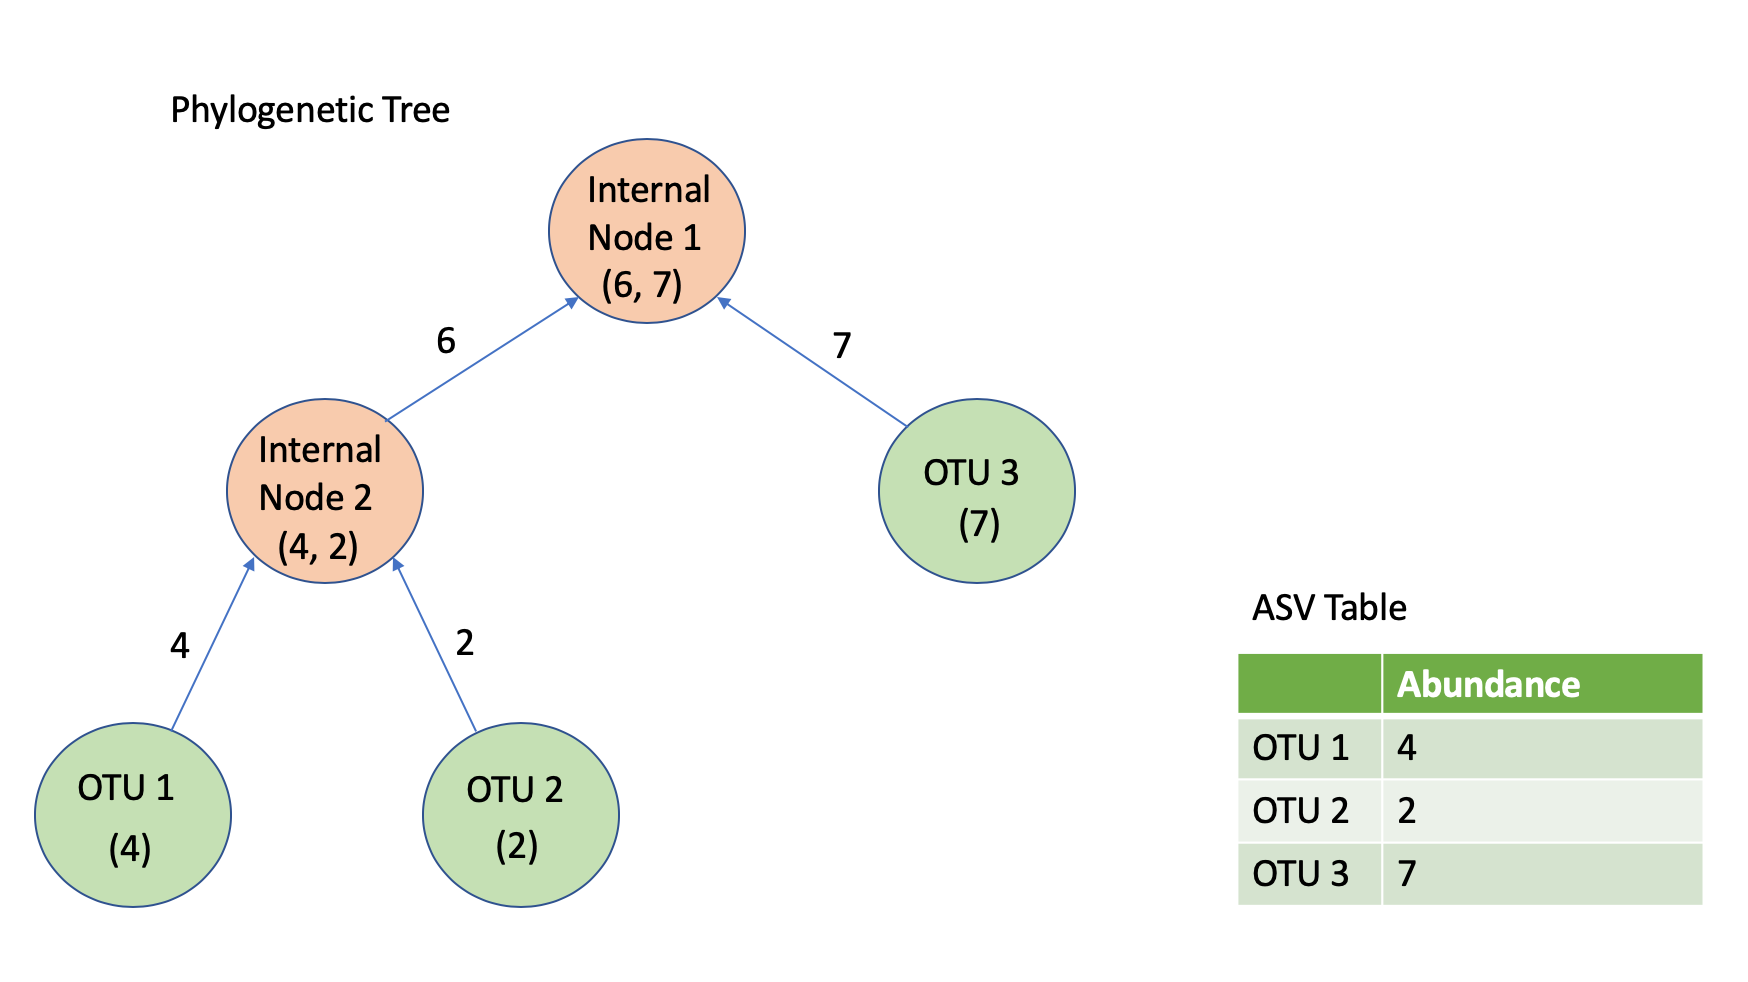
\includegraphics[width=700px]{figure/figure15} \caption{An example of bottom-up propagation of abundance counts}\label{fig:figure15}
\end{figure}
In addition to using calculating counts going left and right at each
internal node, code was also written in Python to determine the
taxonomic rankings of each internal node, based upon the assigned
taxonomies from the RDP for each ASV column in the sequence table.
Figure 5.2 provides a smaller example of this propagation process.
\begin{figure}
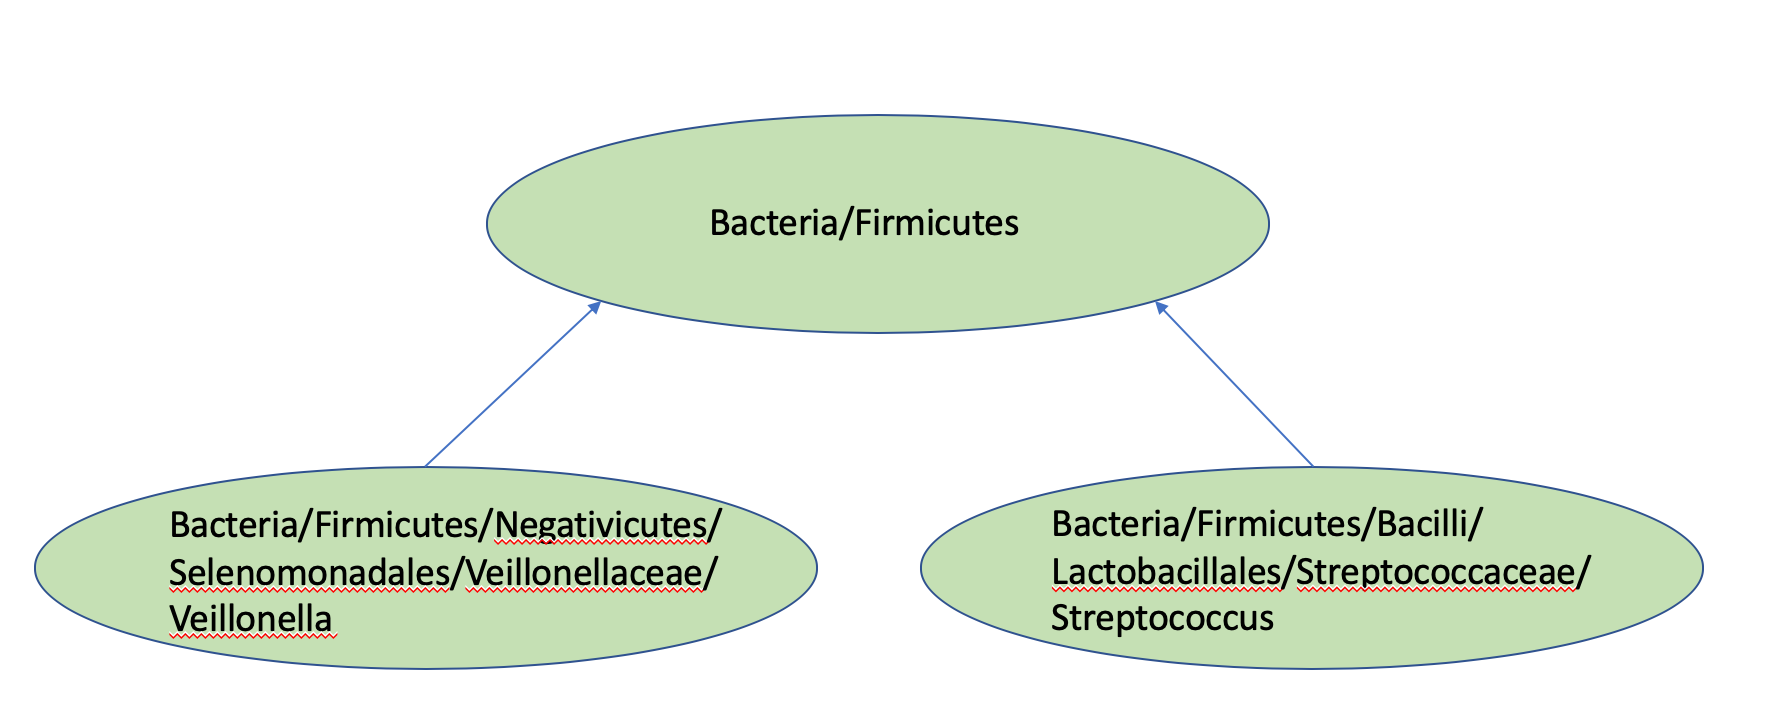
\includegraphics[width=700px]{figure/figure16} \caption{An example of bottom-up propagation of Taxonomies}\label{fig:figure16}
\end{figure}
With calculated counts and taxonomies for each of the internal nodes of
our phylogenetic tree, we then applied a logit mixed-effect binomial
model to each one, using the ``glmer'' function of the R ``lme4''
package (Bates 2015). At each node, we had 370 observations after
filtration for missing values. There were a total of 129 different
patients in our dataset. We incorporated a random effect for patient ID,
and a nested random effect within patientID for sampleDate. We also
included fixed effects for Batch number, transplant Age, gender,
ethnicity, diagnosis, transplant type, graft source, vital status, care
environment, presence of acute graft v. host disease, presence of
chronic graft v. host disease, ANC500 level, and ``preOrPost,'' telling
us if the first sample was taken before or after the transplant date.

The general format of our mixed effects model is as follows:

\(logit(P_{i}(A)) = X_{i}\beta^{(A)} + \gamma_{i}^{(A)} + \epsilon_{it}^{(A)}\)

\(P_{i}(A)\) is the probability of picking the left child of node A for
sample \(i\) at time \(t\).

\(\gamma_{i}^{(A)} = N(0, \sigma_{\gamma}^{2})\)

\(\epsilon_{i}^{(A)} = N(0, \sigma_{\epsilon}^{2})\)

\(for \ i = 1,...,370\)

In most cases, the regression model would fail to converge and provide
meaningful results. However, there were twenty-two different internal
nodes for which our model finished running and identified different
variables to be significant. There were also several instances where
Batch effects were noticed, including four nodes where the only
significant variable was Batch number. The eighteen nodes that
identified significant variables other than Batch are detailed in the
table below, providing their taxonomy, the taxonomies of their children,
and the significant covariates at their node.
\begin{longtable}[]{@{}ccc@{}}
\caption{Significant Variables from Regression on Internal
Nodes}\tabularnewline
\toprule
\begin{minipage}[b]{0.23\columnwidth}\centering\strut
Taxonomy\strut
\end{minipage} & \begin{minipage}[b]{0.46\columnwidth}\centering\strut
Children's Taxonomies\strut
\end{minipage} & \begin{minipage}[b]{0.22\columnwidth}\centering\strut
Significant Variables\strut
\end{minipage}\tabularnewline
\midrule
\endfirsthead
\toprule
\begin{minipage}[b]{0.23\columnwidth}\centering\strut
Taxonomy\strut
\end{minipage} & \begin{minipage}[b]{0.46\columnwidth}\centering\strut
Children's Taxonomies\strut
\end{minipage} & \begin{minipage}[b]{0.22\columnwidth}\centering\strut
Significant Variables\strut
\end{minipage}\tabularnewline
\midrule
\endhead
\begin{minipage}[t]{0.23\columnwidth}\centering\strut
None/NA\strut
\end{minipage} & \begin{minipage}[t]{0.46\columnwidth}\centering\strut
Kingdom/Woesearchaeota, None/NA\strut
\end{minipage} & \begin{minipage}[t]{0.22\columnwidth}\centering\strut
Diagnosis(MDS, Other), Graft Source(Cord, PBPC), Care Environment(2),
ANC500\strut
\end{minipage}\tabularnewline
\begin{minipage}[t]{0.23\columnwidth}\centering\strut
Domain/Bacteria\strut
\end{minipage} & \begin{minipage}[t]{0.46\columnwidth}\centering\strut
Domain/Bacteria, Domain/Bacteria\strut
\end{minipage} & \begin{minipage}[t]{0.22\columnwidth}\centering\strut
Gender(M), Hispanic(Yes), Transplant Type(Auto), Care Environment(2),
preOrPost(pre)\strut
\end{minipage}\tabularnewline
\begin{minipage}[t]{0.23\columnwidth}\centering\strut
Phylum/Firmicutes\strut
\end{minipage} & \begin{minipage}[t]{0.46\columnwidth}\centering\strut
Class/Selenomonadales, Kingdom/Firmicutes\strut
\end{minipage} & \begin{minipage}[t]{0.22\columnwidth}\centering\strut
Gender(M), Hispanic(Unk), Care Environment(2), preOrPost(pre)\strut
\end{minipage}\tabularnewline
\begin{minipage}[t]{0.23\columnwidth}\centering\strut
Domain/Bacteria\strut
\end{minipage} & \begin{minipage}[t]{0.46\columnwidth}\centering\strut
Species/Gemella, Domain/Bacteria\strut
\end{minipage} & \begin{minipage}[t]{0.22\columnwidth}\centering\strut
Transplant Age, Gender(M), Hispanic(Unk), Diagnosis(MDS), Transplant
Type(Auto), preOrPost(pre), CGVHD\strut
\end{minipage}\tabularnewline
\begin{minipage}[t]{0.23\columnwidth}\centering\strut
Order/Ruminococcaceae\strut
\end{minipage} & \begin{minipage}[t]{0.46\columnwidth}\centering\strut
Order/Ruminococcaceae, Order/Ruminococcaceae\strut
\end{minipage} & \begin{minipage}[t]{0.22\columnwidth}\centering\strut
Hispanic(Yes), Graft Source(BM/PBPC)\strut
\end{minipage}\tabularnewline
\begin{minipage}[t]{0.23\columnwidth}\centering\strut
Domain/Bacteria\strut
\end{minipage} & \begin{minipage}[t]{0.46\columnwidth}\centering\strut
Domain/Bacteria, Kingdom/Firmicutes\strut
\end{minipage} & \begin{minipage}[t]{0.22\columnwidth}\centering\strut
Hispanic(Yes), AGVHD\strut
\end{minipage}\tabularnewline
\begin{minipage}[t]{0.23\columnwidth}\centering\strut
Kingdom/Firmicutes\strut
\end{minipage} & \begin{minipage}[t]{0.46\columnwidth}\centering\strut
Kingdom/Firmicutes, Order/Erysipelotrichaceae\strut
\end{minipage} & \begin{minipage}[t]{0.22\columnwidth}\centering\strut
Graft Source(Cord Blood), Care Environment(2), ANC500\strut
\end{minipage}\tabularnewline
\begin{minipage}[t]{0.23\columnwidth}\centering\strut
Order/Erysipelotrichaceae\strut
\end{minipage} & \begin{minipage}[t]{0.46\columnwidth}\centering\strut
Order/Erysipelotrichaceae, Order/Erysipelotrichaceae\strut
\end{minipage} & \begin{minipage}[t]{0.22\columnwidth}\centering\strut
Care Environment(3)\strut
\end{minipage}\tabularnewline
\begin{minipage}[t]{0.23\columnwidth}\centering\strut
Class/Lactobacillales\strut
\end{minipage} & \begin{minipage}[t]{0.46\columnwidth}\centering\strut
Class/Lactobacillales, Class/Lactobacillales\strut
\end{minipage} & \begin{minipage}[t]{0.22\columnwidth}\centering\strut
Hispanic(Yes), preOrPost(pre)\strut
\end{minipage}\tabularnewline
\begin{minipage}[t]{0.23\columnwidth}\centering\strut
Kingdom/Firmicutes\strut
\end{minipage} & \begin{minipage}[t]{0.46\columnwidth}\centering\strut
Order/Erysipelotrichaceae, Kingdom/Firmicutes\strut
\end{minipage} & \begin{minipage}[t]{0.22\columnwidth}\centering\strut
preOrPost(pre)\strut
\end{minipage}\tabularnewline
\begin{minipage}[t]{0.23\columnwidth}\centering\strut
Order/Lactobacillaceae\strut
\end{minipage} & \begin{minipage}[t]{0.46\columnwidth}\centering\strut
Family/Lactobacillus, Order/Lactobacillaceae\strut
\end{minipage} & \begin{minipage}[t]{0.22\columnwidth}\centering\strut
Transplant Type(Auto), ANC500\strut
\end{minipage}\tabularnewline
\begin{minipage}[t]{0.23\columnwidth}\centering\strut
Family/Streptococcus\strut
\end{minipage} & \begin{minipage}[t]{0.46\columnwidth}\centering\strut
Family/Streptococcus, Family/Streptococcus\strut
\end{minipage} & \begin{minipage}[t]{0.22\columnwidth}\centering\strut
Diagnosis(Other), CGVHD\strut
\end{minipage}\tabularnewline
\begin{minipage}[t]{0.23\columnwidth}\centering\strut
Family/Streptococcus\strut
\end{minipage} & \begin{minipage}[t]{0.46\columnwidth}\centering\strut
Family/Streptococcus, Family/Streptococcus\strut
\end{minipage} & \begin{minipage}[t]{0.22\columnwidth}\centering\strut
Transplant Age, Gender(M), Diagnosis(MDS, Other), Graft Source(Cord
Blood)\strut
\end{minipage}\tabularnewline
\begin{minipage}[t]{0.23\columnwidth}\centering\strut
Family/Bacteroides\strut
\end{minipage} & \begin{minipage}[t]{0.46\columnwidth}\centering\strut
Family/Bacteroides, Family/Bacteroides\strut
\end{minipage} & \begin{minipage}[t]{0.22\columnwidth}\centering\strut
Transplant Age, Hispanic(Unknown), Transplant Type(Allo-DLI)\strut
\end{minipage}\tabularnewline
\begin{minipage}[t]{0.23\columnwidth}\centering\strut
Family/Streptococcus\strut
\end{minipage} & \begin{minipage}[t]{0.46\columnwidth}\centering\strut
Family/Streptococcus, Family/Streptococcus\strut
\end{minipage} & \begin{minipage}[t]{0.22\columnwidth}\centering\strut
Graft Source(BM/PBPC, PBPC), CGVHD\strut
\end{minipage}\tabularnewline
\begin{minipage}[t]{0.23\columnwidth}\centering\strut
Family/Bifidobacterium\strut
\end{minipage} & \begin{minipage}[t]{0.46\columnwidth}\centering\strut
Family/Bifidobacterium, Family/Bifidobacterium\strut
\end{minipage} & \begin{minipage}[t]{0.22\columnwidth}\centering\strut
Gender(M), Hispanic(Yes), Transplant Type(Auto), Graft Source(Cord
Blood, PBPC), AGVHD\strut
\end{minipage}\tabularnewline
\begin{minipage}[t]{0.23\columnwidth}\centering\strut
Family/Streptococcus\strut
\end{minipage} & \begin{minipage}[t]{0.46\columnwidth}\centering\strut
Family/Streptococcus, Family/Streptococcus\strut
\end{minipage} & \begin{minipage}[t]{0.22\columnwidth}\centering\strut
AGVHD\strut
\end{minipage}\tabularnewline
\begin{minipage}[t]{0.23\columnwidth}\centering\strut
Family/Bacteroides\strut
\end{minipage} & \begin{minipage}[t]{0.46\columnwidth}\centering\strut
Family/Bacteroides, Family/Bacteroides\strut
\end{minipage} & \begin{minipage}[t]{0.22\columnwidth}\centering\strut
Diagnosis(Other), Transplant Type(Auto), Care Environment(2)\strut
\end{minipage}\tabularnewline
\bottomrule
\end{longtable}
Common variables identified across taxonomic rankings include ethnicity,
graft source, care environment, diagnosis, transplant type, and presence
of acute and chronic graft vs.~host disease.

\chapter*{Conclusion}\label{conclusion}
\addcontentsline{toc}{chapter}{Conclusion}

Overall, our work from this year gave us much insight into the
methodology required to understand and process microbiome data, as well
as revealed the potential behind new methodologies for the visualization
and analysis of associations between patient information and microbiome
compositions.

In terms of future directions for our project, there are many avenues
that we can take. With respect to processing, we can investigate the use
of different filtration parameters in our initial generation of our ASV
table.

For visualizations and simple linear regressions, we could also try to
determine new summary statistics that still effectively represent the
dynamics of the microbiome over time, but are less resistant to the
addition and deletion of data.

With respect to our phylogenetic tree decomposition, it would be useful
to repeat our procedure with either fewer variables in our mixed effects
model, or with more data. We see that our results are relatively sparse,
particularly at nodes that occur lower in our phylogenetic tree. With
more data, our counts would be higher at a larger number of internal
nodes, thus giving us the ability to fit regression models for more than
just twenty-two of them. With more results, we could also analyze the
output of our regression along chains of related nodes, thus controlling
for inter-node variation. There is also potential that functionality
instead of phylogeny might be a better way to characterize the relations
between microbiota. Instead of building a tree solely based upon
taxonomies, it would also be interesting to use a tree based upon
microbial functional groups instead, to have a clearer indication of the
relationship between microbiome functions.

Ultimately, our methodology shows much promise for the identification of
connections between patient recovery from leukemia and their
microbiomes.

\backmatter

\chapter*{References}\label{references}
\addcontentsline{toc}{chapter}{References}

\markboth{References}{References}

\noindent

\setlength{\parindent}{-0.20in} \setlength{\leftskip}{0.20in}
\setlength{\parskip}{8pt}

\hypertarget{refs}{}
\hypertarget{ref-angel2000}{}
Angel, E. (2000). \emph{Interactive computer graphics : A top-down
approach with opengl}. Boston, MA: Addison Wesley Longman.

\hypertarget{ref-angel2001}{}
Angel, E. (2001a). \emph{Batch-file computer graphics : A bottom-up
approach with quicktime}. Boston, MA: Wesley Addison Longman.

\hypertarget{ref-angel2002a}{}
Angel, E. (2001b). \emph{Test second book by angel}. Boston, MA: Wesley
Addison Longman.


% Index?

\end{document}
